\documentclass[11pt,]{article}
\usepackage[left=1in,top=1in,right=1in,bottom=1in]{geometry}
\newcommand*{\authorfont}{\fontfamily{phv}\selectfont}
\usepackage[]{mathpazo}


  \usepackage[T1]{fontenc}
  \usepackage[utf8]{inputenc}



\usepackage{abstract}
\renewcommand{\abstractname}{}    % clear the title
\renewcommand{\absnamepos}{empty} % originally center

\renewenvironment{abstract}
 {{%
    \setlength{\leftmargin}{0mm}
    \setlength{\rightmargin}{\leftmargin}%
  }%
  \relax}
 {\endlist}

\makeatletter
\def\@maketitle{%
  \newpage
%  \null
%  \vskip 2em%
%  \begin{center}%
  \let \footnote \thanks
    {\fontsize{18}{20}\selectfont\raggedright  \setlength{\parindent}{0pt} \@title \par}%
}
%\fi
\makeatother




\setcounter{secnumdepth}{3}

\usepackage{longtable,booktabs}

\usepackage{graphicx,grffile}
\makeatletter
\def\maxwidth{\ifdim\Gin@nat@width>\linewidth\linewidth\else\Gin@nat@width\fi}
\def\maxheight{\ifdim\Gin@nat@height>\textheight\textheight\else\Gin@nat@height\fi}
\makeatother
% Scale images if necessary, so that they will not overflow the page
% margins by default, and it is still possible to overwrite the defaults
% using explicit options in \includegraphics[width, height, ...]{}
\setkeys{Gin}{width=\maxwidth,height=\maxheight,keepaspectratio}

\title{Análisis Morfométrico fluvial de la cuenca del Soco por medio del uso de
sotfware de código abierto  }



\author{\Large Isaac De La Rosa\vspace{0.05in} \newline\normalsize\emph{Estudiante de la Licenciatura en Geografia Mención Representación
Espacial en la Universidad Autónoma de Santo Domingo (UASD)}  }


\date{}

\usepackage{titlesec}

\titleformat*{\section}{\normalsize\bfseries}
\titleformat*{\subsection}{\normalsize\itshape}
\titleformat*{\subsubsection}{\normalsize\itshape}
\titleformat*{\paragraph}{\normalsize\itshape}
\titleformat*{\subparagraph}{\normalsize\itshape}

\titlespacing{\section}
{0pt}{36pt}{0pt}
\titlespacing{\subsection}
{0pt}{36pt}{0pt}
\titlespacing{\subsubsection}
{0pt}{36pt}{0pt}





\newtheorem{hypothesis}{Hypothesis}
\usepackage{setspace}

\makeatletter
\@ifpackageloaded{hyperref}{}{%
\ifxetex
  \PassOptionsToPackage{hyphens}{url}\usepackage[setpagesize=false, % page size defined by xetex
              unicode=false, % unicode breaks when used with xetex
              xetex]{hyperref}
\else
  \PassOptionsToPackage{hyphens}{url}\usepackage[unicode=true]{hyperref}
\fi
}

\@ifpackageloaded{color}{
    \PassOptionsToPackage{usenames,dvipsnames}{color}
}{%
    \usepackage[usenames,dvipsnames]{color}
}
\makeatother
\hypersetup{breaklinks=true,
            bookmarks=true,
            pdfauthor={Isaac De La Rosa (Estudiante de la Licenciatura en Geografia Mención Representación
Espacial en la Universidad Autónoma de Santo Domingo (UASD))},
             pdfkeywords = {Geomorfología fluvial, Morfometría de Cuenca, Análisis Morfométrico,
Cuenca del Soco},  
            pdftitle={Análisis Morfométrico fluvial de la cuenca del Soco por medio del uso de
sotfware de código abierto},
            colorlinks=true,
            citecolor=blue,
            urlcolor=blue,
            linkcolor=magenta,
            pdfborder={0 0 0}}
\urlstyle{same}  % don't use monospace font for urls

% set default figure placement to htbp
\makeatletter
\def\fps@figure{htbp}
\makeatother

\usepackage{pdflscape} \newcommand{\blandscape}{\begin{landscape}}
\newcommand{\elandscape}{\end{landscape}} \usepackage{float}
\floatplacement{figure}{H}
\newcommand{\beginsupplement}{ \setcounter{table}{0} \renewcommand{\thetable}{S\arabic{table}} \setcounter{figure}{0} \renewcommand{\thefigure}{S\arabic{figure}} }


% add tightlist ----------
\providecommand{\tightlist}{%
\setlength{\itemsep}{0pt}\setlength{\parskip}{0pt}}

\begin{document}
	
% \pagenumbering{arabic}% resets `page` counter to 1 
%
% \maketitle

{% \usefont{T1}{pnc}{m}{n}
\setlength{\parindent}{0pt}
\thispagestyle{plain}
{\fontsize{18}{20}\selectfont\raggedright 
\maketitle  % title \par  

}

{
   \vskip 13.5pt\relax \normalsize\fontsize{11}{12} 
\textbf{\authorfont Isaac De La Rosa} \hskip 15pt \emph{\small Estudiante de la Licenciatura en Geografia Mención Representación
Espacial en la Universidad Autónoma de Santo Domingo (UASD)}   

}

}








\begin{abstract}

    \hbox{\vrule height .2pt width 39.14pc}

    \vskip 8.5pt % \small 

\noindent El análisis realizado a la cuenca del Soco arroja resultados
impresionantes, basandose en la descripción de la morfometría fluvial de
la Cuenca y como una ciencia complementaria de la geografía física, la
geomorfología ha sido una de las mas importantes al momento de crear una
perspectiva real del relieve, siendo este util para explicar causas y
consecuencias de movimientos y poder describir los mismos. La cuenca del
Soco inicia entre las subregiones Yuma y Higüamo, con desembocadura en
la boca del soco. Se comprueba en los perfiles longitudinales los cursos
concavos y los cursos convexos. se también comprueba que la curva e
integral hipsométrica está asociada a factores evolutivos de las
regiones que posee el relieve. De forma notoria, se observa Dentro de
este encontramos la geomorfología fluvial, que como etimológicamnte se
indica, es la encargada de describir los procesos fluviales en la
litosfera, asi como tambien sus causas y consecuencias en su paso por la
corteza terrestre, pero existe poca bibliografía científica sobre
morfometría fluvial dominicana. De una forma notoria, Muchas fuentes
afirman que el funcionamiento de una cuenca se asemeja al de un colector
que recibe la precipitación y la convierte en escurrimiento superficial
o sub superficial; esta transformación depende de las condiciones
climáticas y las características físicas de la cuenca. El soco tiene
como área unos 988.62 km2 y un perimetro de 227.63 km, siendo esta la
cuenca mas grande de la region este, esta logra una elevacion maxima de
646.96m, la elevación media 136.34m y la elevación mínima 0.032 m, dicha
cuenca localizada en la región este del país. Estos resultados son
provocados para demostrar la actual información de la la morfometría
fluvial de la Cuenca en cuestión. La República Dominicana con el paso de
los años va quedando en el tiempo al ofrecer datos de tal importancia
como son los antes vistos, y para la realización de trabajos de análisis
morfométrico futuros, o análisis geodésicos, biológicos o geológicos, es
importante tener datos de fuente confiable y segura con datos reales.


\vskip 8.5pt \noindent \emph{Keywords}: Geomorfología fluvial, Morfometría de Cuenca, Análisis Morfométrico,
Cuenca del Soco \par

    \hbox{\vrule height .2pt width 39.14pc}



\end{abstract}


\vskip 6.5pt


\noindent  \section{Introducción}\label{introducciuxf3n}

Seamos geógrafos o aspirantes a serlo, es importante conocer las
características físicas de una cuenca de drenaje, las cuales revisten
gran importancia para la realización de estudios geomorfológicos,
hidrológicos y geotécnicos, ya que influyen en el desarrollo de
múltiples procesos fluviales y en el riesgo de inundación morfometría de
cuenca. Si bien es cierto que cada vez que se hace un estudio de este
tipo o relacionado a este, es en cierto sentido intermiable por la poca
informacion ofrecida por las partes encargadas. (Busnelli \& Horta,
2014), aunque en este artículo tendremos la exepción.

La cuenca el río Soco es una de las mas importantes en el este de dicho
pais, la cual comprende desde la parte norte de la región este hasta la
parte sur de dicha región, políticamente comenzando desde la Provincia
de El Seibo y la Provincia de Hato Mayor del rey, en las zonas muy
forestales y altas de la cordillera del Seibo (cordillera Oriental), y
dicha cuenca sera el punto de concentración de nuestra investigación.
Posee una forma en cierto sentido pensando el punto de desemboque.

Reivindicar la geomorfología, es decir, los procesos y formas abióticos,
en este caso, como valor en sí mismo del sistema fluvial y como clave de
conservación y restauración constituye una innovación en nuestro país,
donde el desconocimiento geomorfológico en el ámbito ambiental es muy
grave, donde muchas veces la geomorfología no se considera (como ocurre
en muchos estudios de impacto) y no es que se infravalore, sino que
directamente no existe o se desprecia. (Ollero et al., 2011).

Lo que vemos en este análisis morfométrico fluvial son datos provocados
de fuentes de código libre, realizandose en el Soco para hallazgos y
contribuciones a la ciencia con mas información útil compartida, ya sea
el primer trabajo de esta area geomorfológoica o no.

Imporante a tomar en cuenta que el concepto de Horton-Strahler ha sido
importante en la geomorfología de las cuencas fluviales; describe
propiedades de escala e identifica GIUH, pero también ha atraído
críticas, porque depende del área de umbral S, que se utiliza para
extraer la red de canales de los modelos digitales de elevación (MDE),
de la posición de la salida y del escaso número de ratios utilizados
para identificar las leyes de escala. Para superar estas limitaciones,
este artículo propone nuevos índices independientes de S y que tienen
propiedades similares a las relaciones de Horton-Strahler.(Moussa,
2009).

La geomorfología regional, definida como ciencia que se ocupa de
describir y explicar la distribución espacial de las formas del terreno
a escala regional y subregional, ha sido considerada por la
planificación física y la ordenación del territorio más clásicas, como
la única disciplina capaz de analizar las ``líneas maestras'' que
definen el carácter complejo del territorio y del paisaje.

La utilización del relieve como base física para la delimitación y
definición de unidades territoriales integradas, básicas para gestionar
el territorio y sus recursos, ha constituido además uno de los métodos
tradicionalmente empleados por algunas de las disciplinas ambientales
que en mayor medida han contribuido al acercamiento de la planificación
física clásica hacia la nueva ordenación integral; es el caso de la
Ecología del Paisaje, la Ecología Humana y la Geografía
Ambiental.(Muñoz-Rojas, Carrasco González, \& Pedraza Gilsanz, 2009).

Este trabajo se centra en la cuenca del soco, como objetivo: su
morfometría, tantos aspectos sean conocidos, realizado con apoyo de
softwares libres y scripts adaptados al área de estudio, la cuenca del
Soco. También, se inquiere sobre la existencia de una relación entre:
los perfiles longitudinales e índice de concavidad con la litología de
la cuenca; la relación entre los parámetros morfométricos con las
características litológica y si hay factores que se asocien con la curva
e integral hipsométricas de la cuenca.Por medio de parámetros
morfométricos se busca identificar qué forma tienen la cuenca y su red
de drenaje. De igual manera, se trata de comprender como se organiza la
red de drenaje; y, tras el estudio de la cuenca y su red de drenaje, se
indaga si se producen ciertros movimientos de reorganización en ellas.
Al realizar estas investigación nos preguntamos ¿Cual es el orden
concreto de la cuenca del Soco? ¿Qué otra información obtenemos al
investigar esta cuenca? ¿Podrían utilizarse sus aguas para hacer una
presa o represa en ella?

\section{Area de Estudio}\label{area-de-estudio}

El presente estudio fue realizado en la cuenca del río Soco, ubicada en
la zona Este de la República Dominicana, con una extensión superficial
de 988.62 km2, siendo esta una de las mas grandes del pais, con forma
ilustrativa a un triangulo isosceles invertido. Dicha cuenca tiene como
rio principal y/o cabecera el río Soco, teniendo su nacimiento en una de
las montañas de la Cordillera del Seibo, al sur de la poblacion de
miches, y desembocando así en la Boca del Soco, donde termina la cuenca
de análisis.

Dicha cuenca pasa por Hato Mayor Del Rey (70,141 Hab) El Seibo (97,144
Hab) La Romana (139,671 Hab) y San Pedro de Macorís (217, 141). cuenca
ubicada de Nor Noreste hasta Sur Suroreste, comprendiendo desde
elevaciónes superiores de la cordillera del Seibo hasta la Llanura
costera del caribe, Vertiendo sus aguas en el mar caribe.

\section{Metodología}\label{metodologuxeda}

Para la realización de estas operaciones se utilizaron operaciones de
análisis morfométrico de redes de drenaje y cuenca de los paquetes de
software de código abierto GRASS GIS, utilizando como medio de
interpretación y organización cuantitativa y/o cualitativa de
información R como entorno de programación (``RStudio,'' 2012)
implementado y desglosado en la computadora de uso familiar.

Lo utilizado para la caputura de resultados fue de varios addons, y
apertura de mapas y análisis en R, donde se hizo de los mismos para asi
extraer resultados, creando primero una región donde se guardaron los
datos recogidos en el analisis de la cuenca, uso el cual se le dió en
orden de metodos.

Dentro de GRASS GIS fueron utilizados otros paquetes para la óptima
comprensión de datos, con la utilización de un modelo digital de
elevacion (para lo siguiente, MDE) de la misión radar del transbordador
espacia Shuttle (Lemos, Souza, \& Rocha, 2004), con altura aproximada a
90 metros para la extracción de información requiriente.

Para extraer la cuenca se utilizó el addon r.water.outlet (Lozar, 2003),
usado también el addon r.vect, lo que llevó a convertir el raster
resultante en vectorial, para así colocacarlo en R. De igual forma se
aplicó el addon r.stream.extract (Jasiewicz, 2011), para lograr extraer
la red de drenaje donde se llevaron a R los resultados del mismo.

En la acumulación de flujo, los parámetros de cuenca del mismo, como
elevación, drenaje, y otros más, fueron calculados a través del addon de
GRASS GIS r.watershed (Lozar, 2003), contando con un umbral acumulado de
82 celdas, en un MDE. Las capas generadas se ingresaron a R al junto de
la libreria ap y al igual manejo con la libreria raster Por
consiguiente, en la orden de red y el análisis hortoniano, se puso en
uso el addon r.stream.extract para producir un mapa de dirección de
flujo. Por otra parte, para la creación de mapas de ordenes de red se
uso el addon r.stream.order (Jasiewicz, 2011), en el cual se usó la
clasificación de de Strahler para el analisis de red de dicha cuenca.

Se utilizaron de igual forma los addons r.info para extraer los valores
máximos y mínimos del orden de red segun Strahler partiendo de un
raster, delimitada la cuenca a traves de la red de drenaje con
r.stream.basins (Jasiewicz, 2011). Para el uso de estadostocas según
orden de red de Horton para las redes de Strahler y Horton, se utilizó
el addon r.stream.stats (Jasiewicz, 2011) en resumen de las
estadísticas.

Luego de la creación de una nueva región de GRASS en R, se llevaron a
números enteros la extensión y la resolución del DEM con las funciones
integerextent y xyvector (José Ramón Martínez Batlle, 2018). También se
llegó a utilizar la herramienta gdalwarp (``GDAL-biblioteca de
abstracción de datos geoespaciales,'' 2005) para extraer la sesión de
GRASS. se usó el addon r.stream.extract, para generar la red de drenaje
y obtener las coordenadas que mas adelante seria convetrtidas a
EPGS:4326 (Jain, 2003), como números enteros con la función my\_trans.
(José Ramón Martínez Batlle, 2020)

Mientras que, para la obtención de los parámetros morfométricos de la
cuenca se utilizó el addon r.basin (Di Leo, 2013). Los vectores
obtenidos son transformados a EPGS:4326 (Jain, 2003) y así siendo vistos
o visualizados con la liobreria leaflet. De igual forma, para explorar
los parámetros de la cuenca fue utilizada la libreria readr.

Para el cálculo de los índices de concavidad y los perfiles
longitudinales, en primer lugar, se extajeron los cursos mas largos de
la cuenca en cuestión a través de la función LfpNetwork, para luego
emplear la función LfpProfilesConcavity, dicha función arrojó los
índices de concavidad para los cursos mas largos, y así mismo, sus
perfiles longitudinales.

En la última parte de realización para el cálculo de la curva y la
integral hipsométrica de la cuenca, en primer lugar, lo realizado fue
representar las cuencas con las librerias sp y mapview; y en segundo
lugar, calcular la integral y cuva hipsométrica mediante el uso de la
función HypsoIntCurve (José Ramón Martínez Batlle, 2018).

\section{Resultados}\label{resultados}

En este estudio realizado a la cuenca del Soco utilizando el script
reproducible, revela información que facilita el análisis y comprensión
de la cuenca. vierase de manera agrupada como de forma desagregada. Por
consiguiente, se presentan de manera resumida, las caracteristicas
morfométricas principales de la cuenca en cuestion y su red de drenaje.

Como se muestra en la tabla abajo descrita, la cuenca del Soco tiene
como área unos 988.62 km2 y un perímetro de 227.63 km, siendo esta la
cuenca mas grande de la región este, esta logra alcanzar una elevación
máxima de 646.96m, la elevación media siendo de 136.34m y la elevación
mínima de 0.032, con uno de los relieves mas heterogeneos e irregulares
antes analizados.

\begin{longtable}[]{@{}ll@{}}
\caption{\label{tablasiete}Parámetros morfométricos de la Cuenca del
Soco}\tabularnewline
\toprule
\begin{minipage}[b]{0.66\columnwidth}\raggedright\strut
Párametros\strut
\end{minipage} & \begin{minipage}[b]{0.28\columnwidth}\raggedright\strut
Valores\strut
\end{minipage}\tabularnewline
\midrule
\endfirsthead
\toprule
\begin{minipage}[b]{0.66\columnwidth}\raggedright\strut
Párametros\strut
\end{minipage} & \begin{minipage}[b]{0.28\columnwidth}\raggedright\strut
Valores\strut
\end{minipage}\tabularnewline
\midrule
\endhead
\begin{minipage}[t]{0.66\columnwidth}\raggedright\strut
Easting Centroid of basin\strut
\end{minipage} & \begin{minipage}[t]{0.28\columnwidth}\raggedright\strut
489195.00\strut
\end{minipage}\tabularnewline
\begin{minipage}[t]{0.66\columnwidth}\raggedright\strut
Northing Centroid of basin\strut
\end{minipage} & \begin{minipage}[t]{0.28\columnwidth}\raggedright\strut
2072655.00\strut
\end{minipage}\tabularnewline
\begin{minipage}[t]{0.66\columnwidth}\raggedright\strut
Rectangle containing basin N-W\strut
\end{minipage} & \begin{minipage}[t]{0.28\columnwidth}\raggedright\strut
(`471060', `2092680')``\strut
\end{minipage}\tabularnewline
\begin{minipage}[t]{0.66\columnwidth}\raggedright\strut
Rectangle containing basin S-E\strut
\end{minipage} & \begin{minipage}[t]{0.28\columnwidth}\raggedright\strut
``(`513630', `2039760')''\strut
\end{minipage}\tabularnewline
\begin{minipage}[t]{0.66\columnwidth}\raggedright\strut
Area of basin {[}km2{]}\strut
\end{minipage} & \begin{minipage}[t]{0.28\columnwidth}\raggedright\strut
989.801775\strut
\end{minipage}\tabularnewline
\begin{minipage}[t]{0.66\columnwidth}\raggedright\strut
Perimeter of basin {[}km{]}\strut
\end{minipage} & \begin{minipage}[t]{0.28\columnwidth}\raggedright\strut
227.636525830754\strut
\end{minipage}\tabularnewline
\begin{minipage}[t]{0.66\columnwidth}\raggedright\strut
Max Elevation {[}m s.l.m.{]}\strut
\end{minipage} & \begin{minipage}[t]{0.28\columnwidth}\raggedright\strut
646.969411439852\strut
\end{minipage}\tabularnewline
\begin{minipage}[t]{0.66\columnwidth}\raggedright\strut
Min Elevation {[}m s.l.m.{]}\strut
\end{minipage} & \begin{minipage}[t]{0.28\columnwidth}\raggedright\strut
0.0326075545062636\strut
\end{minipage}\tabularnewline
\begin{minipage}[t]{0.66\columnwidth}\raggedright\strut
Elevation Difference {[}m{]}\strut
\end{minipage} & \begin{minipage}[t]{0.28\columnwidth}\raggedright\strut
646.9368038853457\strut
\end{minipage}\tabularnewline
\begin{minipage}[t]{0.66\columnwidth}\raggedright\strut
Mean Elevation\strut
\end{minipage} & \begin{minipage}[t]{0.28\columnwidth}\raggedright\strut
136.3463\strut
\end{minipage}\tabularnewline
\begin{minipage}[t]{0.66\columnwidth}\raggedright\strut
Mean Slope\strut
\end{minipage} & \begin{minipage}[t]{0.28\columnwidth}\raggedright\strut
4.65\strut
\end{minipage}\tabularnewline
\begin{minipage}[t]{0.66\columnwidth}\raggedright\strut
Length of Directing Vector {[}km{]}\strut
\end{minipage} & \begin{minipage}[t]{0.28\columnwidth}\raggedright\strut
33.6112628742212\strut
\end{minipage}\tabularnewline
\begin{minipage}[t]{0.66\columnwidth}\raggedright\strut
Prevalent Orientation {[}degree from north, counterclockwise{]}\strut
\end{minipage} & \begin{minipage}[t]{0.28\columnwidth}\raggedright\strut
1.250701649253028\strut
\end{minipage}\tabularnewline
\begin{minipage}[t]{0.66\columnwidth}\raggedright\strut
Compactness Coefficient\strut
\end{minipage} & \begin{minipage}[t]{0.28\columnwidth}\raggedright\strut
6.412284389087794\strut
\end{minipage}\tabularnewline
\begin{minipage}[t]{0.66\columnwidth}\raggedright\strut
Circularity Ratio\strut
\end{minipage} & \begin{minipage}[t]{0.28\columnwidth}\raggedright\strut
0.2400347916120\strut
\end{minipage}\tabularnewline
\begin{minipage}[t]{0.66\columnwidth}\raggedright\strut
Topological Diameter\strut
\end{minipage} & \begin{minipage}[t]{0.28\columnwidth}\raggedright\strut
,120.0\strut
\end{minipage}\tabularnewline
\begin{minipage}[t]{0.66\columnwidth}\raggedright\strut
Elongation Ratio\strut
\end{minipage} & \begin{minipage}[t]{0.28\columnwidth}\raggedright\strut
0.4103977285869175\strut
\end{minipage}\tabularnewline
\begin{minipage}[t]{0.66\columnwidth}\raggedright\strut
Shape Factor\strut
\end{minipage} & \begin{minipage}[t]{0.28\columnwidth}\raggedright\strut
,11.44258120713636\strut
\end{minipage}\tabularnewline
\begin{minipage}[t]{0.66\columnwidth}\raggedright\strut
``Concentration Time (Giandotti, 1934) {[}hr{]}\strut
\end{minipage} & \begin{minipage}[t]{0.28\columnwidth}\raggedright\strut
12.561301584730437\strut
\end{minipage}\tabularnewline
\begin{minipage}[t]{0.66\columnwidth}\raggedright\strut
Length of Mainchannel {[}km{]}\strut
\end{minipage} & \begin{minipage}[t]{0.28\columnwidth}\raggedright\strut
86.501616819\strut
\end{minipage}\tabularnewline
\begin{minipage}[t]{0.66\columnwidth}\raggedright\strut
Mean slope of mainchannel {[}percent{]}\strut
\end{minipage} & \begin{minipage}[t]{0.28\columnwidth}\raggedright\strut
1.0508578295624251\strut
\end{minipage}\tabularnewline
\begin{minipage}[t]{0.66\columnwidth}\raggedright\strut
Mean hillslope length {[}m{]}\strut
\end{minipage} & \begin{minipage}[t]{0.28\columnwidth}\raggedright\strut
311.9917\strut
\end{minipage}\tabularnewline
\begin{minipage}[t]{0.66\columnwidth}\raggedright\strut
Elevation Difference {[}m{]}\strut
\end{minipage} & \begin{minipage}[t]{0.28\columnwidth}\raggedright\strut
646.9368038853457\strut
\end{minipage}\tabularnewline
\begin{minipage}[t]{0.66\columnwidth}\raggedright\strut
Magnitudo,\strut
\end{minipage} & \begin{minipage}[t]{0.28\columnwidth}\raggedright\strut
289.0\strut
\end{minipage}\tabularnewline
\begin{minipage}[t]{0.66\columnwidth}\raggedright\strut
Max order (Strahler)\strut
\end{minipage} & \begin{minipage}[t]{0.28\columnwidth}\raggedright\strut
5\strut
\end{minipage}\tabularnewline
\begin{minipage}[t]{0.66\columnwidth}\raggedright\strut
Number of streams\strut
\end{minipage} & \begin{minipage}[t]{0.28\columnwidth}\raggedright\strut
421\strut
\end{minipage}\tabularnewline
\begin{minipage}[t]{0.66\columnwidth}\raggedright\strut
Total Stream Length {[}km{]}\strut
\end{minipage} & \begin{minipage}[t]{0.28\columnwidth}\raggedright\strut
815.5888\strut
\end{minipage}\tabularnewline
\begin{minipage}[t]{0.66\columnwidth}\raggedright\strut
First order stream frequency\strut
\end{minipage} & \begin{minipage}[t]{0.28\columnwidth}\raggedright\strut
0.2919776538085113\strut
\end{minipage}\tabularnewline
\begin{minipage}[t]{0.66\columnwidth}\raggedright\strut
Drainage Density {[}km/km\^{}2{]}\strut
\end{minipage} & \begin{minipage}[t]{0.28\columnwidth}\raggedright\strut
0.8239920563892704\strut
\end{minipage}\tabularnewline
\begin{minipage}[t]{0.66\columnwidth}\raggedright\strut
Bifurcation Ratio (Horton)\strut
\end{minipage} & \begin{minipage}[t]{0.28\columnwidth}\raggedright\strut
4.2453\strut
\end{minipage}\tabularnewline
\begin{minipage}[t]{0.66\columnwidth}\raggedright\strut
Length Ratio (Horton)\strut
\end{minipage} & \begin{minipage}[t]{0.28\columnwidth}\raggedright\strut
2.4703\strut
\end{minipage}\tabularnewline
\begin{minipage}[t]{0.66\columnwidth}\raggedright\strut
Area ratio (Horton)\strut
\end{minipage} & \begin{minipage}[t]{0.28\columnwidth}\raggedright\strut
4.6963\strut
\end{minipage}\tabularnewline
\begin{minipage}[t]{0.66\columnwidth}\raggedright\strut
Slope ratio (Horton)\strut
\end{minipage} & \begin{minipage}[t]{0.28\columnwidth}\raggedright\strut
1.3574\strut
\end{minipage}\tabularnewline
\bottomrule
\end{longtable}

\begin{figure}
\centering
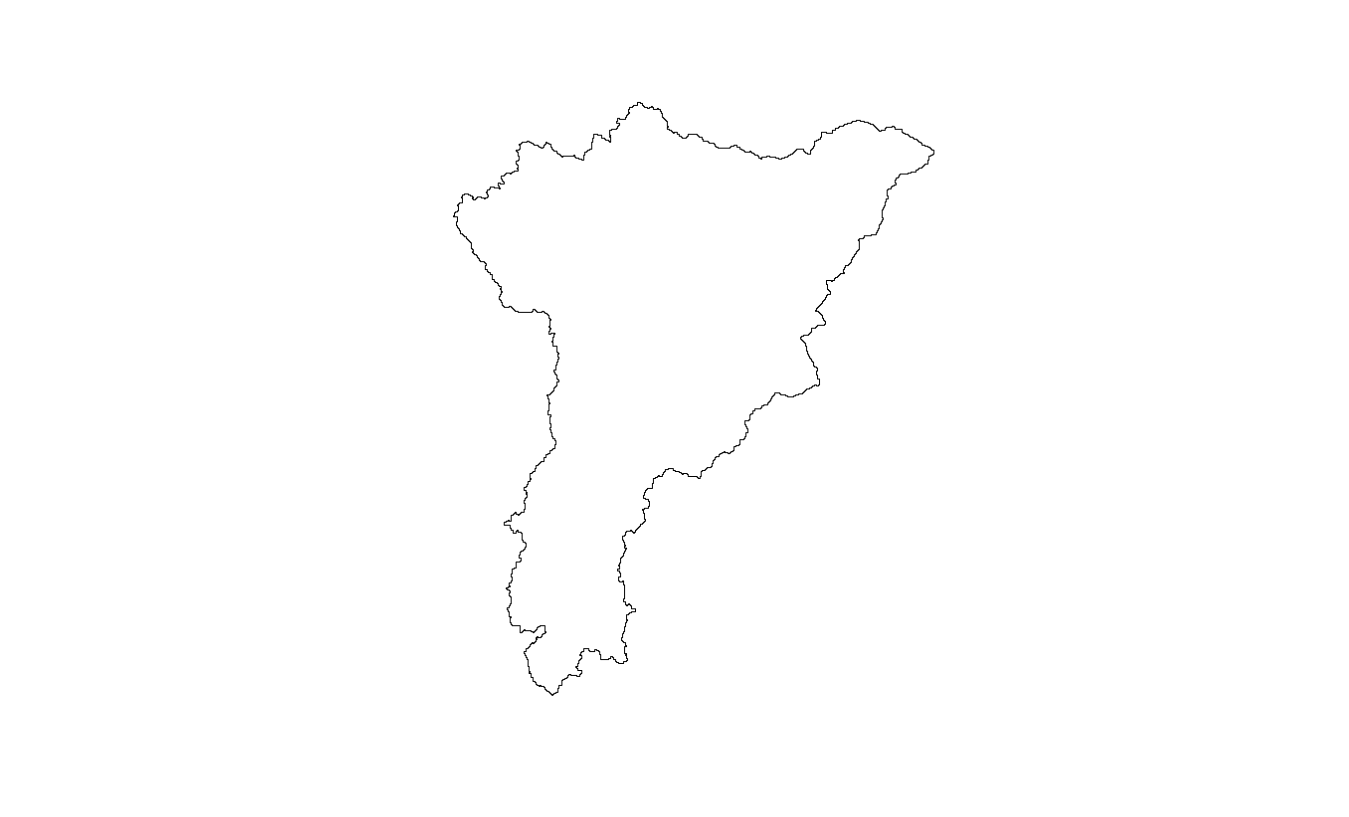
\includegraphics{form cu soc.png}
\caption{Forma de la Cuenca del Soco\label{mapacero}}
\end{figure}

Observandose la figura la forma de la cuenca es ciertamente triangular,
con la parte mas ancha en el norte y la punta de la figura en el sur con
su desembocadura. Así mismo, los párametros de coeficiente de
compacidad, forma de la cuenca y razón de elongación, nos dan la
confirmación de la forma triangular de la cuenca en cuestión (ver tabla
\ref{tablanueve}). Mientras que la red de drenaje de la cuenca se pueden
ver drenajes acumulados y de cierta forma informales, siendo densa en
ramificaciones muy regulares tal vemos en la cuenca media alta, al sur;
debido a que relive se denota accidentado y a que la composición del
material encontrado en la sierra del seibo, elevaciones territoriales
importantes en la región y donde nace, por consiguiente, la cuenca del
Soco.

\begin{figure}
\centering
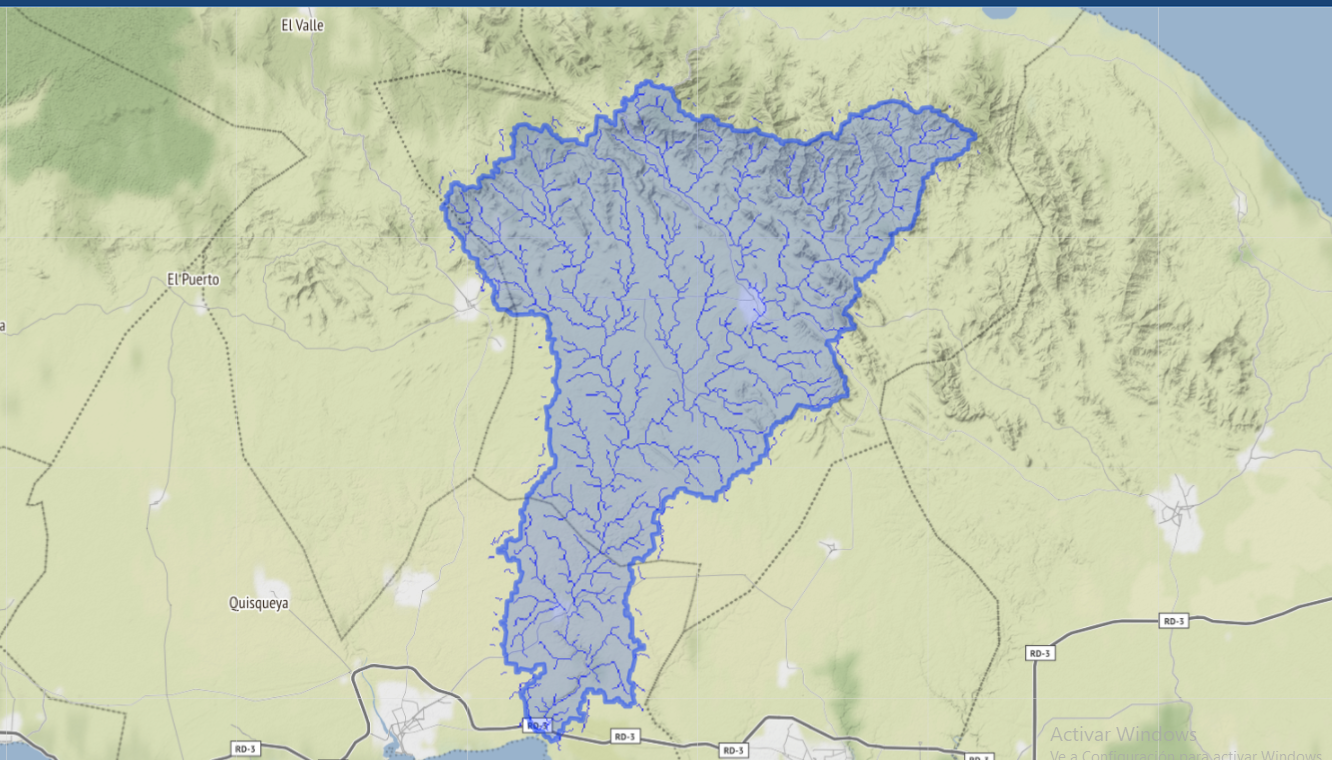
\includegraphics[width=0.70000\textwidth]{denaje.png}
\caption{Red de Drenaje de la Cuenca del Soco\label{mapanueve}}
\end{figure}

La red de drenaje de la cuenca, Según Srahler, presenta un total de 461
redes (ver tabla \ref{tablauno}), y se organiza por ordenes desde el
numero 1 hasta la numero 5

\begin{figure}
\centering
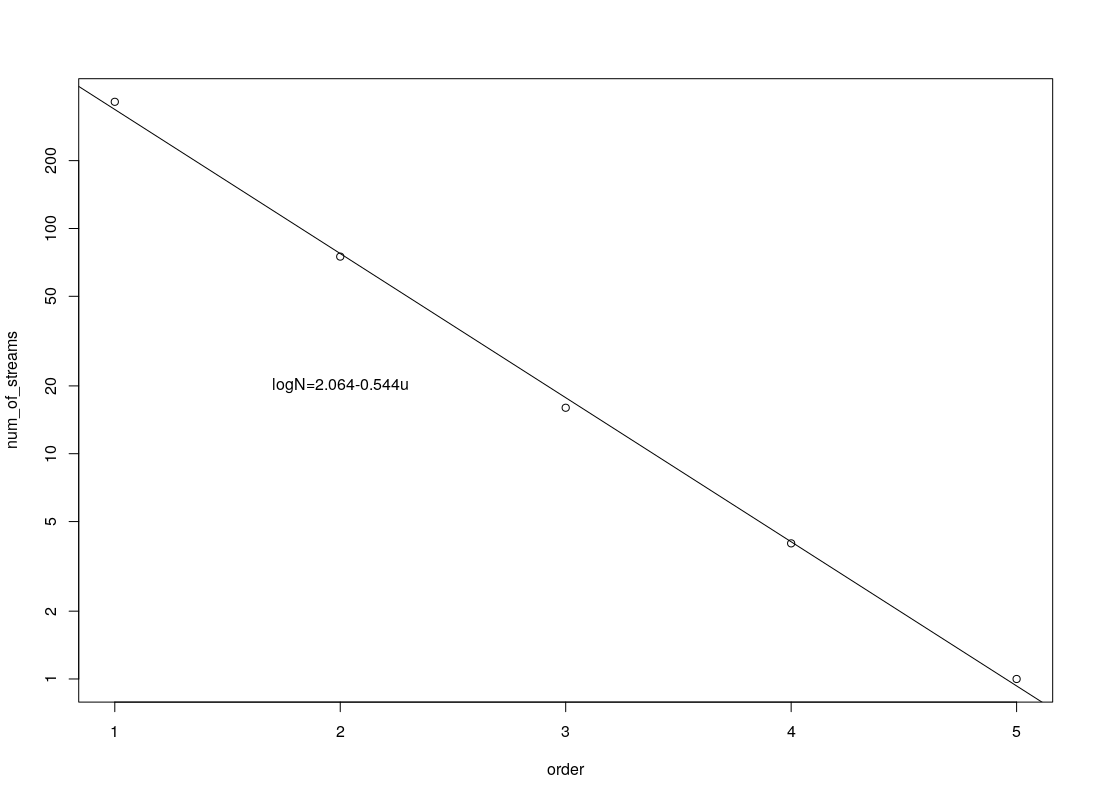
\includegraphics[width=0.70000\textwidth]{num redes razon bif.png}
\caption{Número de ordenes de Redes y Razón de
Bifurcación\label{mapaseis}}
\end{figure}

\begin{figure}
\centering
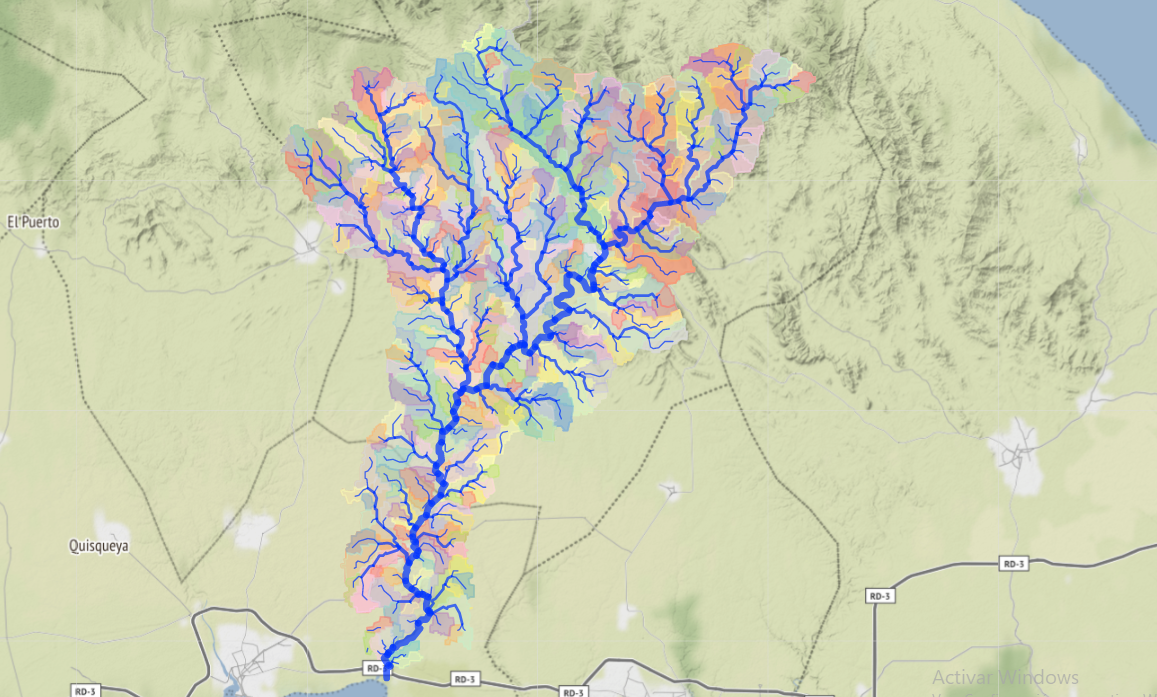
\includegraphics[width=0.70000\textwidth]{drenaje segun orden.png}
\caption{Red de Drenaje según su Orden de Red en la Cuenca del
Soco\label{mapadiez}}
\end{figure}

Donde éstas redes de drenaje de orden uno hasta orden cinco organizados
de forma concatenada, van dando como afluentes sus aguas a un curso
fluvial mayor hasta llegar al curso principal; las de orden dos, que
suman un total de 75, se ve una reducción en el número de redes,
presentando cierto aumento en el area del orden y descenso en las redes
de drenaje de redes, de orden 3 se encontraron 16m de orden 4 se pudo
encontrar 5 y por consiguiente, en el orden 5 solo se encontró uno solo.

En un análisis se prevee que contenga captura fluvial en los cursos mas
largos de drenaje, los cuales generaron los perfiles longitudinales y se
obtuvieron los índices de concavidad, la gran mayoría mostraron ser
positivos a la concavidad, otros salieron negativos a ella, tratandose
de unos 6 con este caso.(ver figura \ref{mapaocho}).

\begin{figure}
\centering
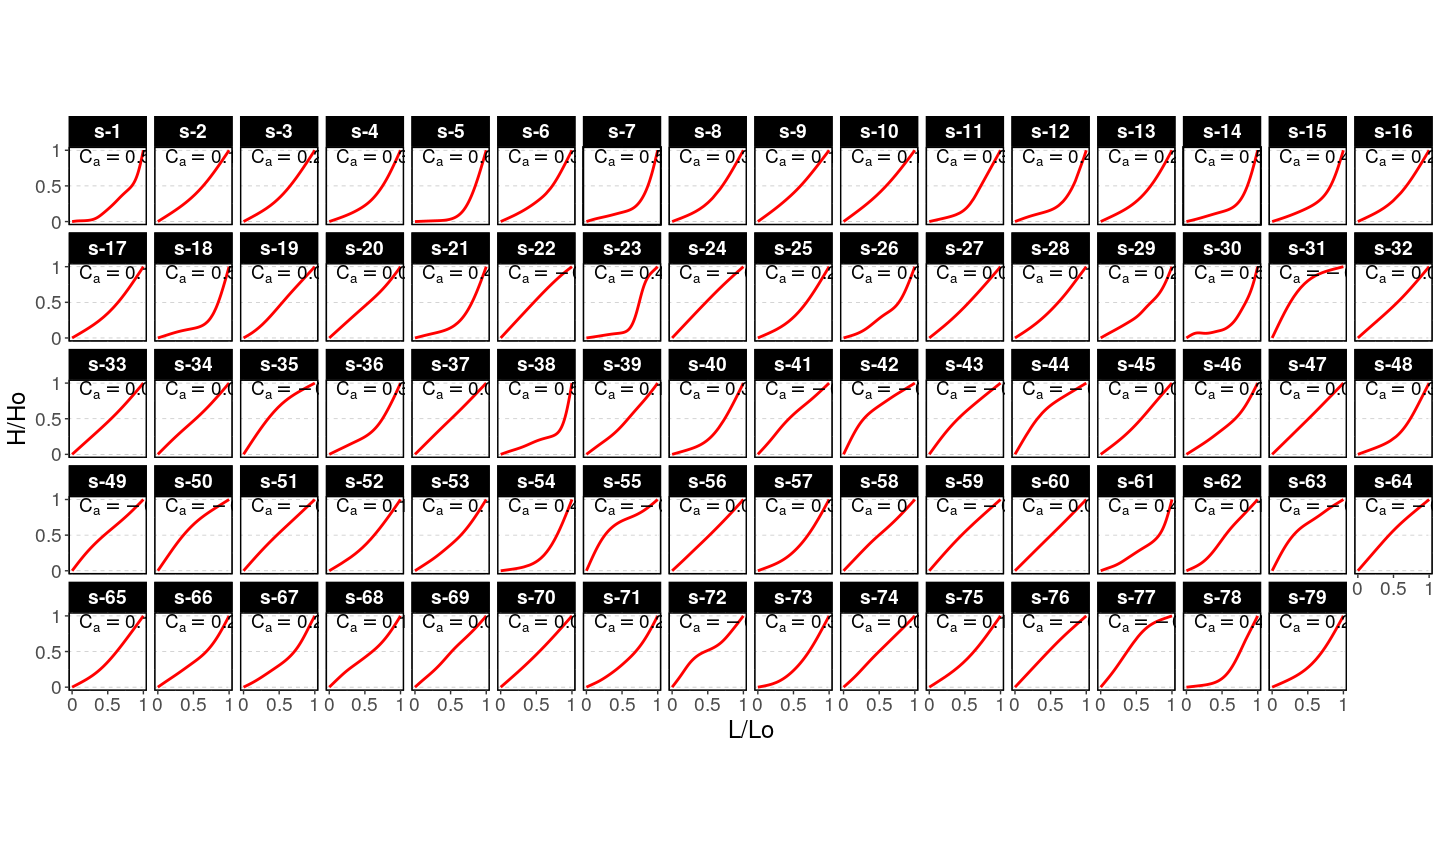
\includegraphics[width=0.70000\textwidth]{mas largos.png}
\caption{Perfiles Longitudinlaes e indices de concavidad de los cursos
mas largos de la cuenca del Soco\label{mapaocho}}
\end{figure}

Los parámetros morfométricos que se obtuvieron (ver tabla
\ref{tablasiete}) incluyendo coeficiente de compacidad que indica que la
forma de la superficial de la cuenca de acuerdo con su delimitación y el
predominio en su escorrentía, es muy alargada; pero tomando en cuenta el
parámetro forma de la cuenca genera un índice el cual indica que la
cuenca, además de ser muy alargada, es bastante ensanchada por las áreas
de cuenca media y cuenca alta.

De los cursos mas largos, se destaca el número 5 (ver figura
\ref{mapados}), siendo este meramente el rio cabecera, el rio soco, el
cual desemboca en la boca del soco al sur de la cuenca, el curso se
mueve englobado de norte a sur, presentando líneas concavas que
facilitan su curso, creando meandros en su recorrido, políticamente pasa
por 3 provincias, libros del servicio Geológico Nacional del 2019
muestran un cauce formado por piedra caliza y conglomerados, sin
presencia de clinoformas, mientras que presenta anchura en su lecho en
la parte baja de la cuenca,.

Por otra parte, en los perfiles podemos apreciar varias líneas convexas,
contando con 18 redes convexas, de órdenes menores, llámense 2,3,4, en
la parte norte de la cuenca y a los alfuentes de los alrededores, la
mayoría desde el número 31 en adelante. La razón de bifurcación mostrada
en los resultado de la ejecución (ver tabla \ref{tablasiete}), muestrean
una constancia en los números y en el área como tal.

También están los cursos casi rectilíneos como son los caso del los
cursos numero 24, 37 y 47 con índices de concavidad menores a 0.18,
rectilíneos a mas de 50\%. la cuencas del soco tiene 461 ríos de órdenes
contables, lo que la convierte en una de las cuencas mas grandes e
importantes de la nación.(ver tabla \ref{tablauno})

\begin{longtable}[]{@{}llllll@{}}
\caption{\label{tablauno} Estadísticas de los ordenes de red de la
Cuenca del Soco}\tabularnewline
\toprule
Pedido máximo & Tot.N.str. & Tot.str.len. & Tot.area. & Dr.dens &
Str.freq.\tabularnewline
\midrule
\endfirsthead
\toprule
Pedido máximo & Tot.N.str. & Tot.str.len. & Tot.area. & Dr.dens &
Str.freq.\tabularnewline
\midrule
\endhead
(núm) & (núm) & (km) & (km2) & (km / km2) & (núm / km2)\tabularnewline
5 & 461 & 827.6249 & 988.6235 & 0,8371 & 0.4663\tabularnewline
\bottomrule
\end{longtable}

Las estadísticas que son generadas sobre la curva y la integral
hipsométrica obtuvieron 75 resultados para los cursos que en red de
orden 2 todos con gran similitudes y por lo tanto, pocas diferencias que
comentar, todos con curvas moderadas, las cuales muestran un proceso de
evolución históricamente/gemorfológicamente normales.(ver tabla
\ref{tablaocho} y ver mapa \label{mapados})

Para los cursos de agua que estan asignados en orden número 3 de la
cuenca del soco, se produjeron 17 resultados donde los valores mas altos
tuvieron cierta evolución en cuanto a elevación se refiere, donde todos
se realizaron de forma uniforme y con un poco de elevación media.

\section{Discusión}\label{discusiuxf3n}

Con dichos datos anteriormente mencionados, consecuentes a la cuenca del
Soco, hemos respondido preguntas planteadas de investigación en marcha
sobre que tan lejos esta el inicio de la cuenca, forma de la misma y su
red de drenaje, organización de esta y la relacion de los perfiles
longitudinales y su índice de de concavidad junto a la litología en la
cuenca. Sin embargo, las preguntas concernientes a la relación de los
parámetros de la cuenca con la litología en la cuenca, como la
importancia de esta cuenca para el lugar situado, no han han sido
respondidas a razón de la falta de información e investigaciones, al
pasar de los años no se ha provisto de información concreta sobre la
cuenca del soco. Tal es que la información encontrada fue sobre la Boca
del Soco dada por el Servicio Geologico Nacional.

La cuenca tiene forma de triangulo isosceles invertido, y la forma de la
red de drenaje es dendrítrica. Dicha cuenca produce esta forma en zonas
de relieve notoriamente heterogeneo, como se presenta la parte de cuenca
alta; los cursos de agua van desarrollandose libremente y no van
dependiendo de un control estructural. Es normal en los ordenes de red
de las cuencas, desde el orden 1 al orden 5, principalmente en las de
orden 5, tipos de rocas y relieve mas heterogeneo, producto al arrastre
de la escorrentía desde afluentes a este mas arriba.

Según estudiosos como Summerfield, explican que la razon de bifurcación
que se encuentra entre 3 y 5, da a lugar que la litología del área es
semi homogenea. en la tabla \ref{tablasiete} son visibles los valores
ciertamente dentro del mismo rango. Notese como los ordenes 1,2,3 y 4,
mantienen cierta homogeniedad en la litología.

\begin{longtable}[]{@{}llllllll@{}}
\caption{\label{tablasiete}Razones de los parametros hidrograficos segun
su orden de red.}\tabularnewline
\toprule
Order & Bif.rt. & Len.rt. & Area.rt. & Slo.rt. & Grd.rt. & d.dens. &
str.freq.\tabularnewline
\midrule
\endfirsthead
\toprule
Order & Bif.rt. & Len.rt. & Area.rt. & Slo.rt. & Grd.rt. & d.dens. &
str.freq.\tabularnewline
\midrule
\endhead
1 & 4.8667 & 2.7139 & 0.0000 & 1.6406 & 1.6100 & 0.6762 &
0.6175\tabularnewline
2 & 4.6875 & 2.0492 & 5.1588 & 1.6358 & 2.0326 & 0.3557 &
0.1197\tabularnewline
3 & 4.0000 & 2.0396 & 4.0855 & 1.2922 & 1.6364 & 0.1784 &
0.0293\tabularnewline
4 & 4.0000 & 4.6611 & 4.6057 & 0.8313 & 2.0090 & 0.0790 &
0.0064\tabularnewline
5 & 0.0000 & 0.0000 & 6.2588 & 0.0000 & 0.0000 & 0.0588 &
0.0010\tabularnewline
\bottomrule
\end{longtable}

Los cursos fluviales mas largos de la orden de red encontrados en en
análisis de la cuenca del soco fueron los: 5, 7, 23, 14, 25 y 40, dichos
cursos no se encuentran registrados con nombres directos según lo
investigado en otras fuentes. Sí conocemos que está el rio Soco, Rio
cabecera de la cuenca, siendo este el curso fluvial numero cinco con
alrededor de 61 km de largo, desembocando en la boca del soco, donde
termina la cuenca. Cabe destacar que esta boca tiene costas de manglares
hasta su llegada a la playa, observadas presencialmente desde el puente
que cruza el río.

\begin{figure}
\centering
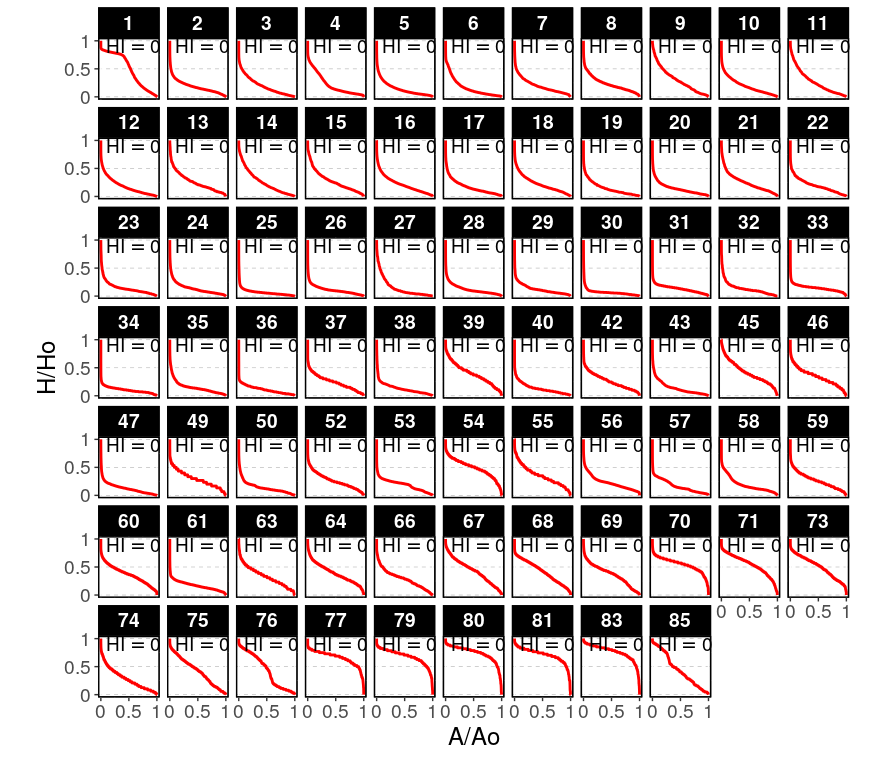
\includegraphics[width=0.70000\textwidth]{c de red o dos.png}
\caption{Cuenca de Orden de Red Numero 2\label{mapados}}
\end{figure}

Comparando los resultados de la vectorial (ver tabla \ref{tablauno}) y
el que se obtuvo con r. basin (ver tabla \ref{tablaocho}), el curso mas
largo es el numero 5, obtenido gracias a la función lfpNetwprk. Por lo
que gracias a la confirmación doble notamos que el río Soco es el curso
mas largo de la cuenca en cuestión.

\begin{longtable}[]{@{}lll@{}}
\caption{\label{tablaocho}Integral Hipsometrica en las cuencas de Orden
2}\tabularnewline
\toprule
ord & cat & Int. Hipso\tabularnewline
\midrule
\endfirsthead
\toprule
ord & cat & Int. Hipso\tabularnewline
\midrule
\endhead
1 & 1 & 0.48838926\tabularnewline
2 & 2 & 0.18193323\tabularnewline
3 & 3 & 0.19445524\tabularnewline
4 & 4 & 0.21762542\tabularnewline
5 & 5 & 0.14295602\tabularnewline
6 & 6 & 0.15991775\tabularnewline
7 & 7 & 0.19598821\tabularnewline
8 & 8 & 0.22972788\tabularnewline
9 & 9 & 0.29999456\tabularnewline
10 & 10 & 0.19312651\tabularnewline
11 & 11 & 0.26362902\tabularnewline
12 & 12 & 0.18092041\tabularnewline
13 & 13 & 0.25637129\tabularnewline
14 & 14 & 0.25578278\tabularnewline
15 & 15 & 0.27399930\tabularnewline
16 & 16 & 0.21718352\tabularnewline
17 & 17 & 0.16731969\tabularnewline
18 & 18 & 0.22313861\tabularnewline
19 & 19 & 0.14558501\tabularnewline
20 & 20 & 0.14253386\tabularnewline
21 & 21 & 0.24687863\tabularnewline
22 & 22 & 0.19453870\tabularnewline
23 & 23 & 0.14312417\tabularnewline
24 & 24 & 0.13588177\tabularnewline
25 & 25 & 0.06656511\tabularnewline
26 & 26 & 0.10905142\tabularnewline
27 & 27 & 0.14094699\tabularnewline
28 & 28 & 0.11947547\tabularnewline
29 & 29 & 0.12154615\tabularnewline
30 & 30 & 0.06694574\tabularnewline
31 & 31 & 0.12986863\tabularnewline
32 & 32 & 0.13214347\tabularnewline
33 & 33 & 0.14299769\tabularnewline
34 & 34 & 0.10321406\tabularnewline
35 & 35 & 0.14836356\tabularnewline
36 & 36 & 0.10991497\tabularnewline
37 & 37 & 0.24081809\tabularnewline
38 & 38 & 0.12914719\tabularnewline
39 & 39 & 0.38783102\tabularnewline
40 & 40 & 0.13000859\tabularnewline
41 & 42 & 0.25771843\tabularnewline
42 & 43 & 0.13739951\tabularnewline
43 & 45 & 0.41175533\tabularnewline
44 & 46 & 0.33664967\tabularnewline
45 & 47 & 0.12660206\tabularnewline
46 & 49 & 0.29142210\tabularnewline
47 & 50 & 0.14173861\tabularnewline
48 & 52 & 0.26207370\tabularnewline
49 & 53 & 0.18704006\tabularnewline
50 & 54 & 0.48698763\tabularnewline
51 & 55 & 0.34952735\tabularnewline
52 & 56 & 0.22693968\tabularnewline
53 & 57 & 0.16492509\tabularnewline
54 & 58 & 0.18884589\tabularnewline
55 & 59 & 0.26409218\tabularnewline
56 & 60 & 0.36586150\tabularnewline
57 & 61 & 0.16777662\tabularnewline
58 & 63 & 0.33413105\tabularnewline
59 & 64 & 0.38969687\tabularnewline
60 & 66 & 0.28774555\tabularnewline
61 & 67 & 0.43177657\tabularnewline
62 & 68 & 0.41594979\tabularnewline
63 & 69 & 0.36691619\tabularnewline
64 & 70 & 0.54537122\tabularnewline
65 & 71 & 0.54050406\tabularnewline
66 & 73 & 0.50115083\tabularnewline
67 & 74 & 0.28375791\tabularnewline
68 & 75 & 0.41880781\tabularnewline
69 & 76 & 0.43451360\tabularnewline
70 & 77 & 0.65887177\tabularnewline
71 & 79 & 0.68029357\tabularnewline
72 & 80 & 0.73798593\tabularnewline
73 & 81 & 0.70710689\tabularnewline
74 & 83 & 0.76043899\tabularnewline
75 & 85 & 0.44416178\tabularnewline
\bottomrule
\end{longtable}

En el área de La curva y la integral hipsométrica se muestra una
repartición de elevaciones de la cuenca (Batlle, 2021), el valor minimo
generado para la integral hipsométrica fue de 0.04. en los cursos mas
curvos tenemos a los números 30 a 35 (ver tabla \ref{tablados}). Los
cursos 73 y 75 son los mas rectilineos y su integral hipsométrica es
moderada por lo que estos cursos han experimentado una evolución lenta
en su elevación.(ver tabla \ref{mapados})

Los cursos propios de la orden de red 3, el curso de mayor valor
numérico (16) muestra una inestable evolución y elevación (ver tabla
\ref{mapacuatro})

\begin{figure}
\centering
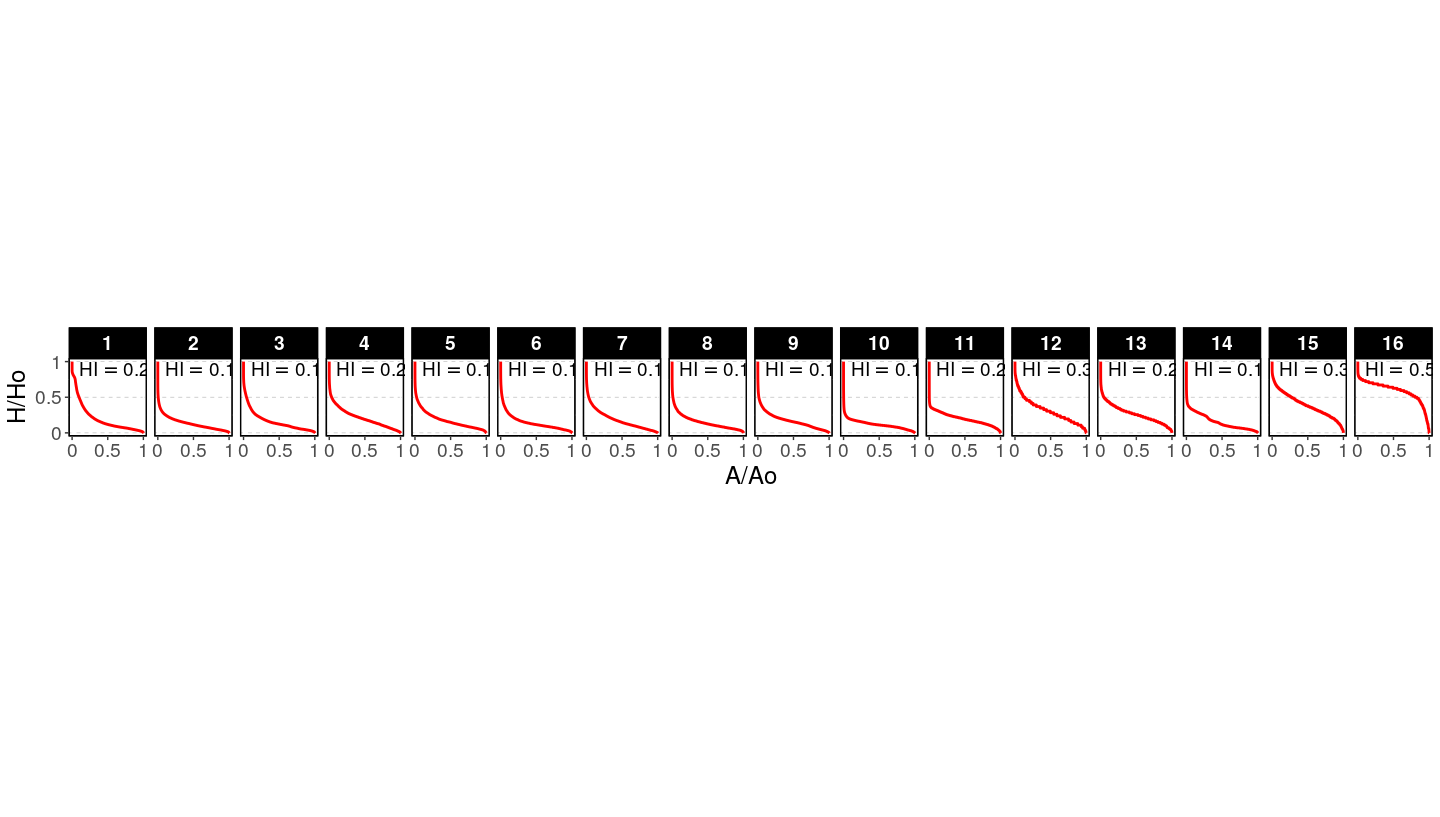
\includegraphics[width=0.70000\textwidth]{cu de red or tres.png}
\caption{Cuenca de Orden de Red Numero Tres\label{mapacuatro}}
\end{figure}

El orden estructurado de la cuenca muestra una afirmacion a la pregunta
sobre la estructura de ordenes de la cuenca del soco, se concluye que es
posible colocar una represa pequeña dedicada a la producción de
electricidad, siempre y cuando se sitúe en área de pendiente semi
inclinada y en el río cabecera, convenientemente en una de sus
confluencias mas cercanas a la desemmbocadura, ya que la pendiente
creada desde la cordillera Oriental llevando aguas a la Llanura Costera
del Caribe, crea una fuerte escorrentía aprovechable.

La cuenca del Soco tiene otras ventajas importantes las cuales se
relaciónan al terreno, y cabe destacar que los terratenientes de esas
areas no suelen utilizar aguas del río para abastecimiento.

Aunque no se pudo hacer una comparación concreta de información obtenida
en el uso de software libre de la cuenca del soco con otras fuentes, el
uso de las mismas fue usado de forma cuantitativamente productiva. Cabe
destacar que toda esta información ha servido como puerta a
investigaciones futuras sobre morfometría fluvial en el país.

Esto crea esperanzas de nuevas investigaciones cercanamente futuras y
ayuda al desarrollo informativo de la Geografia Dominicana, siendo un
reto para el estudio de movimientos geomorfologicos futuros siendo
comparados con los datos de esta investigación.

\section{Agradecimientos}\label{agradecimientos}

A Dios, por otorgar las fuerzas necesarias para realizar lo visto

Al M.A.~Jose Ramon Martinez Batlle, por su paciencia y dedicación al
enseñar con la intención de dejar una marca inolvidable en mi mente.

A mis padres, Angel Maria de la Rosa (Wilden) por enseñarme sobre
redacción y Maireny Esmeralda Caraballo Jimenez, por sus consejos y
ánimos

A mi hermano, Isaias De La Rosa.

A mi mismo, por la fuerza de lo voluntad que gracias a Dios poseo.

\section{Información de soporte}\label{informaciuxf3n-de-soporte}

\begin{longtable}[]{@{}lllll@{}}
\caption{\label{tablados}Tasas de transmisión basadas en el coeficiente
de regresión}\tabularnewline
\toprule
Bif.rt. & Len.rt. & Area.rt & Slo.rt. & Grd.rt.\tabularnewline
\midrule
\endfirsthead
\toprule
Bif.rt. & Len.rt. & Area.rt & Slo.rt. & Grd.rt.\tabularnewline
\midrule
\endhead
4,3627 & 2,5513 & 4.8325 & 1,3319 & 1.8136\tabularnewline
\bottomrule
\end{longtable}

\begin{longtable}[]{@{}lllll@{}}
\caption{\label{tablatres}Relaciones de flujo promediadas con
desviaciones estándar}\tabularnewline
\toprule
Bif.rt. & Len.rt. & Area.rt & Slo.rt. & Grd.rt.\tabularnewline
\midrule
\endfirsthead
\toprule
Bif.rt. & Len.rt. & Area.rt & Slo.rt. & Grd.rt.\tabularnewline
\midrule
\endhead
4,3885 & 2,8660 & 3,4625 & 1,3500 & 1,8220\tabularnewline
0,4546 & 1,2377 & 2,3496 & 0,3823 & 0,2300\tabularnewline
\bottomrule
\end{longtable}

\begin{figure}
\centering
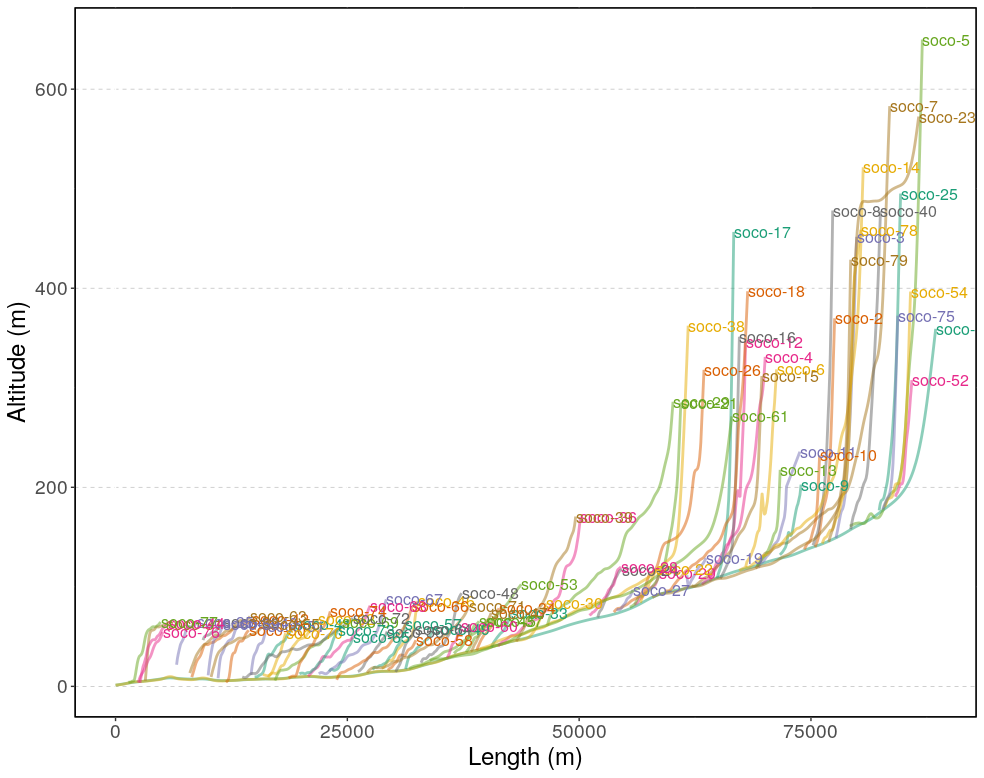
\includegraphics[width=0.50000\textwidth]{perf mas largo.png}
\caption{Perfiles Longitudinales de los cursos mas largos en la Cuenca
del Soco\label{mapauno}}
\end{figure}

\begin{figure}
\centering
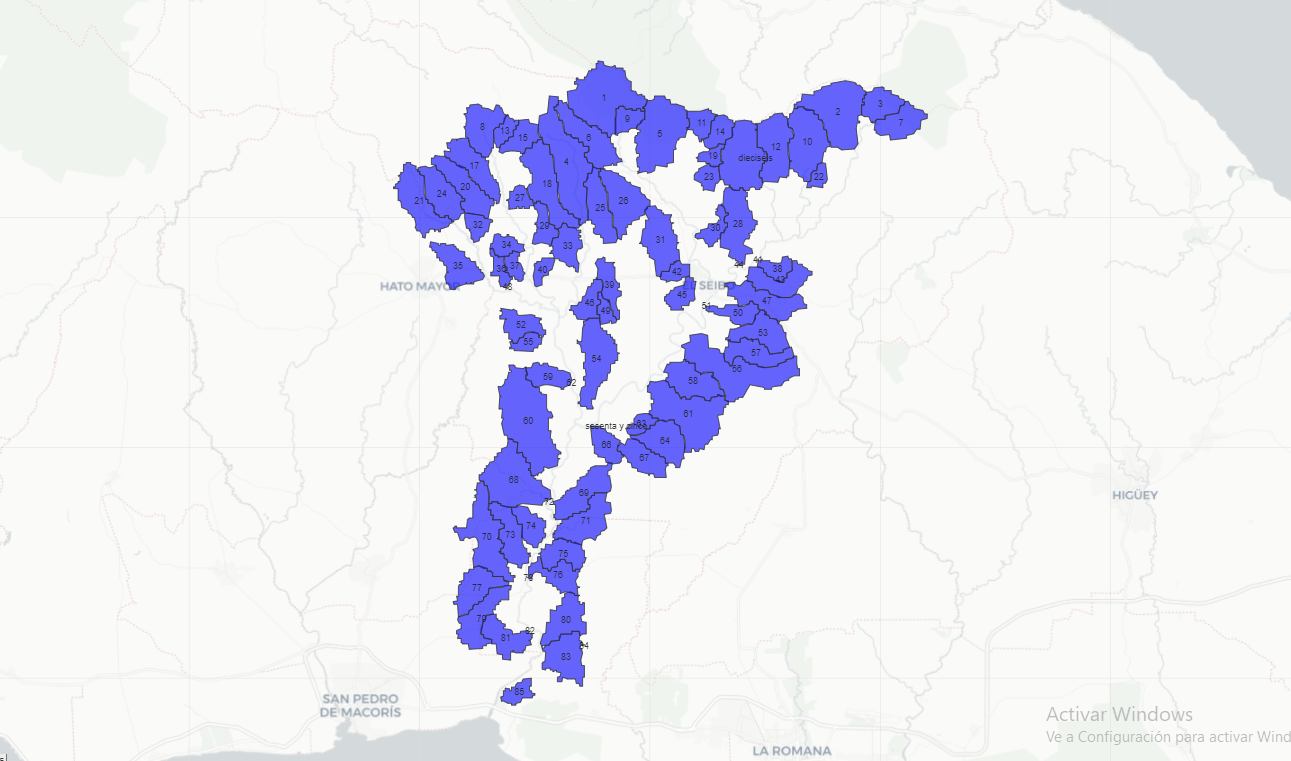
\includegraphics[width=0.70000\textwidth]{cu drena or dos.png}
\caption{Red de Drenaje de orden Dos\label{mapatres}}
\end{figure}

\begin{figure}
\centering
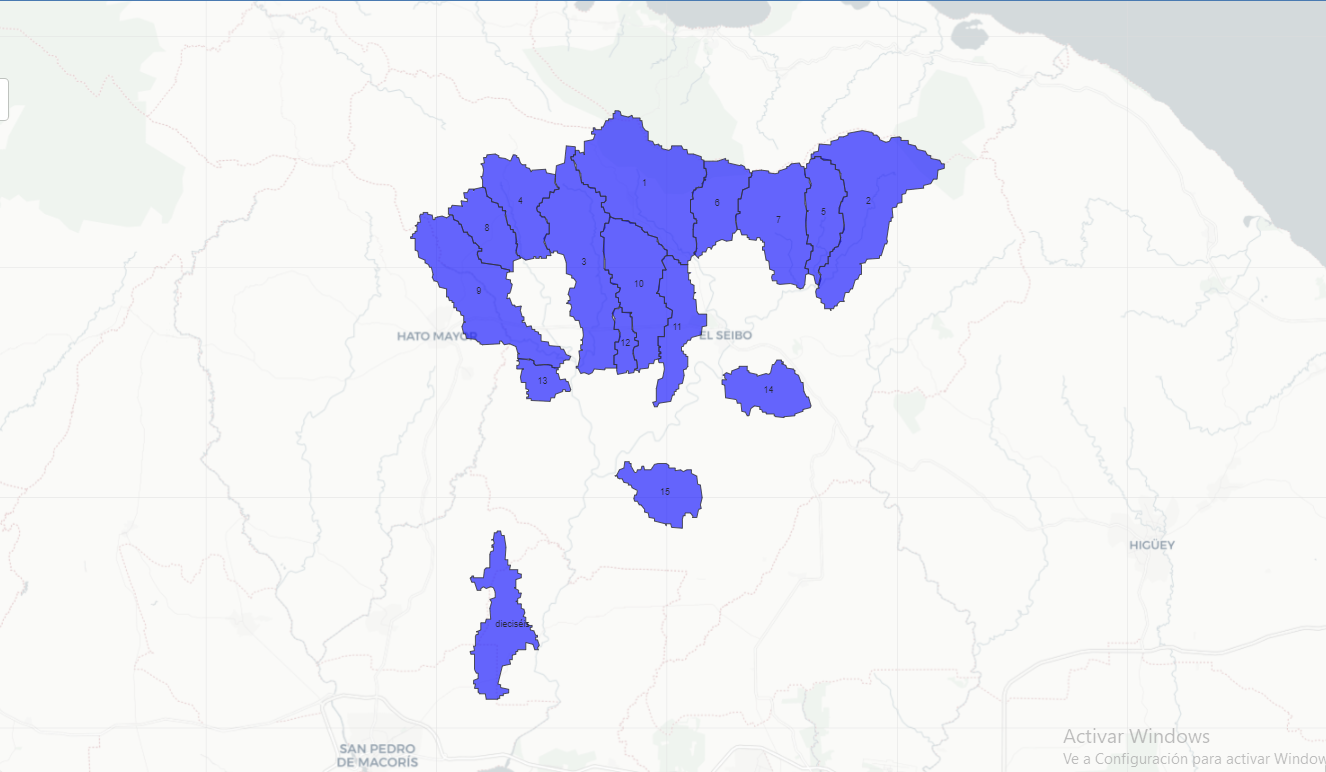
\includegraphics[width=0.70000\textwidth]{cu drena or tres.png}
\caption{Red de Drenaje de orden Dos\label{mapacinco}}
\end{figure}

\begin{figure}
\centering
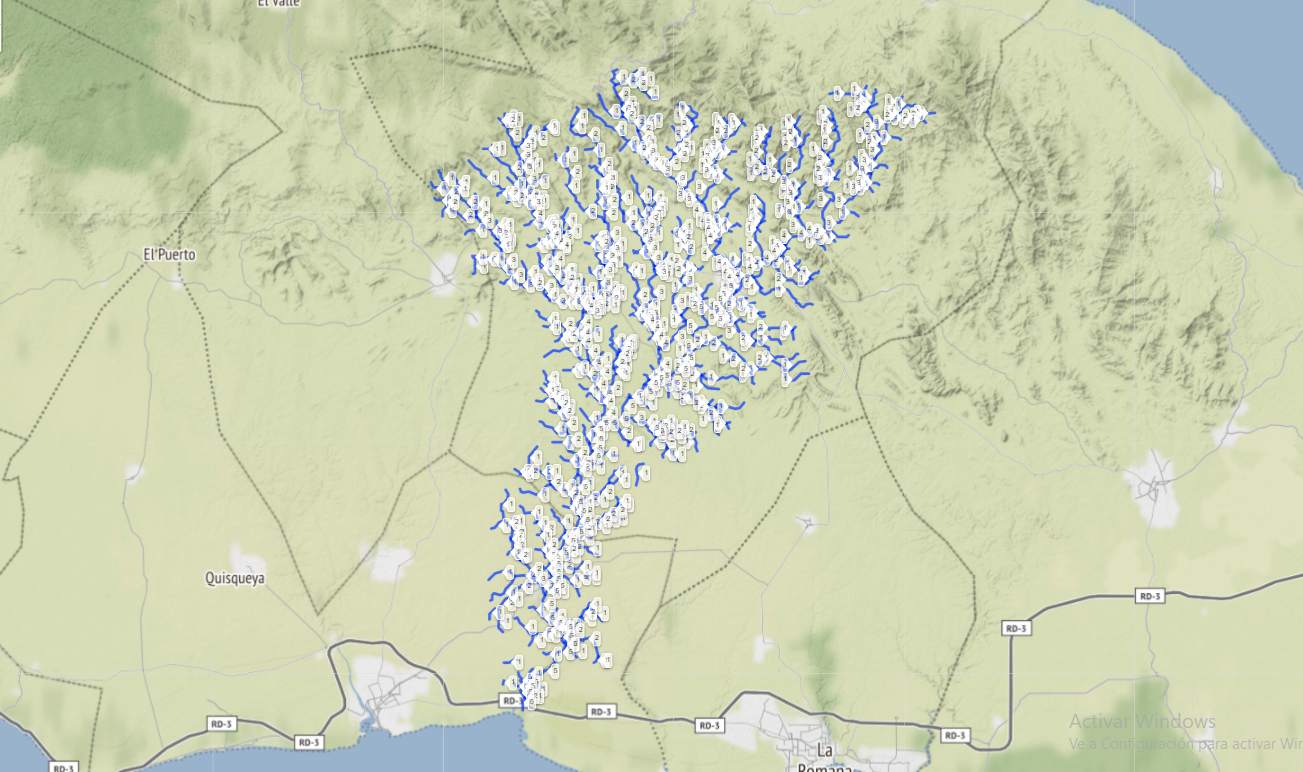
\includegraphics[width=0.70000\textwidth]{unica sim.png}
\caption{Ordenes de Red de la cuenca del Soco con única
Simbología\label{mapasiete}}
\end{figure}

\begin{longtable}[]{@{}llllll@{}}
\caption{\label{tablacuatro}Variables promediadas para cada orden de
red.}\tabularnewline
\toprule
\begin{minipage}[b]{0.12\columnwidth}\raggedright\strut
Order Num\strut
\end{minipage} & \begin{minipage}[b]{0.13\columnwidth}\raggedright\strut
Avg.len (km)\strut
\end{minipage} & \begin{minipage}[b]{0.13\columnwidth}\raggedright\strut
Avg.ar (km2)\strut
\end{minipage} & \begin{minipage}[b]{0.13\columnwidth}\raggedright\strut
Avg.sl (m/m)\strut
\end{minipage} & \begin{minipage}[b]{0.16\columnwidth}\raggedright\strut
Avg.grad. (m/m)\strut
\end{minipage} & \begin{minipage}[b]{0.15\columnwidth}\raggedright\strut
Avg.el.dif (m)\strut
\end{minipage}\tabularnewline
\midrule
\endfirsthead
\toprule
\begin{minipage}[b]{0.12\columnwidth}\raggedright\strut
Order Num\strut
\end{minipage} & \begin{minipage}[b]{0.13\columnwidth}\raggedright\strut
Avg.len (km)\strut
\end{minipage} & \begin{minipage}[b]{0.13\columnwidth}\raggedright\strut
Avg.ar (km2)\strut
\end{minipage} & \begin{minipage}[b]{0.13\columnwidth}\raggedright\strut
Avg.sl (m/m)\strut
\end{minipage} & \begin{minipage}[b]{0.16\columnwidth}\raggedright\strut
Avg.grad. (m/m)\strut
\end{minipage} & \begin{minipage}[b]{0.15\columnwidth}\raggedright\strut
Avg.el.dif (m)\strut
\end{minipage}\tabularnewline
\midrule
\endhead
\begin{minipage}[t]{0.12\columnwidth}\raggedright\strut
1\strut
\end{minipage} & \begin{minipage}[t]{0.13\columnwidth}\raggedright\strut
1.0951\strut
\end{minipage} & \begin{minipage}[t]{0.13\columnwidth}\raggedright\strut
1.6194\strut
\end{minipage} & \begin{minipage}[t]{0.13\columnwidth}\raggedright\strut
0.0218\strut
\end{minipage} & \begin{minipage}[t]{0.16\columnwidth}\raggedright\strut
0.0162\strut
\end{minipage} & \begin{minipage}[t]{0.15\columnwidth}\raggedright\strut
17.6603\strut
\end{minipage}\tabularnewline
\begin{minipage}[t]{0.12\columnwidth}\raggedright\strut
2\strut
\end{minipage} & \begin{minipage}[t]{0.13\columnwidth}\raggedright\strut
2.9720\strut
\end{minipage} & \begin{minipage}[t]{0.13\columnwidth}\raggedright\strut
8.3544\strut
\end{minipage} & \begin{minipage}[t]{0.13\columnwidth}\raggedright\strut
0.0133\strut
\end{minipage} & \begin{minipage}[t]{0.16\columnwidth}\raggedright\strut
0.0100\strut
\end{minipage} & \begin{minipage}[t]{0.15\columnwidth}\raggedright\strut
33.2667\strut
\end{minipage}\tabularnewline
\begin{minipage}[t]{0.12\columnwidth}\raggedright\strut
3\strut
\end{minipage} & \begin{minipage}[t]{0.13\columnwidth}\raggedright\strut
6.0900\strut
\end{minipage} & \begin{minipage}[t]{0.13\columnwidth}\raggedright\strut
34.1317\strut
\end{minipage} & \begin{minipage}[t]{0.13\columnwidth}\raggedright\strut
0.0081\strut
\end{minipage} & \begin{minipage}[t]{0.16\columnwidth}\raggedright\strut
0.0049\strut
\end{minipage} & \begin{minipage}[t]{0.15\columnwidth}\raggedright\strut
31.2500\strut
\end{minipage}\tabularnewline
\begin{minipage}[t]{0.12\columnwidth}\raggedright\strut
4\strut
\end{minipage} & \begin{minipage}[t]{0.13\columnwidth}\raggedright\strut
12.4215\strut
\end{minipage} & \begin{minipage}[t]{0.13\columnwidth}\raggedright\strut
157.2015\strut
\end{minipage} & \begin{minipage}[t]{0.13\columnwidth}\raggedright\strut
0.0063\strut
\end{minipage} & \begin{minipage}[t]{0.16\columnwidth}\raggedright\strut
0.0030\strut
\end{minipage} & \begin{minipage}[t]{0.15\columnwidth}\raggedright\strut
38.2500\strut
\end{minipage}\tabularnewline
\begin{minipage}[t]{0.12\columnwidth}\raggedright\strut
5\strut
\end{minipage} & \begin{minipage}[t]{0.13\columnwidth}\raggedright\strut
57.8980\strut
\end{minipage} & \begin{minipage}[t]{0.13\columnwidth}\raggedright\strut
983.8981\strut
\end{minipage} & \begin{minipage}[t]{0.13\columnwidth}\raggedright\strut
0.0076\strut
\end{minipage} & \begin{minipage}[t]{0.16\columnwidth}\raggedright\strut
0.0015\strut
\end{minipage} & \begin{minipage}[t]{0.15\columnwidth}\raggedright\strut
87.0000\strut
\end{minipage}\tabularnewline
\bottomrule
\end{longtable}

\begin{longtable}[]{@{}llllll@{}}
\caption{\label{tablacinco}Desviación estandar para las estadísticas
según orden de red}\tabularnewline
\toprule
\begin{minipage}[b]{0.13\columnwidth}\raggedright\strut
Order Num\strut
\end{minipage} & \begin{minipage}[b]{0.13\columnwidth}\raggedright\strut
Std.len (km)\strut
\end{minipage} & \begin{minipage}[b]{0.13\columnwidth}\raggedright\strut
Std.ar (km2)\strut
\end{minipage} & \begin{minipage}[b]{0.13\columnwidth}\raggedright\strut
Std.sl (m/m)\strut
\end{minipage} & \begin{minipage}[b]{0.15\columnwidth}\raggedright\strut
Std.grad (m/m)\strut
\end{minipage} & \begin{minipage}[b]{0.15\columnwidth}\raggedright\strut
Std.el.dif (m)\strut
\end{minipage}\tabularnewline
\midrule
\endfirsthead
\toprule
\begin{minipage}[b]{0.13\columnwidth}\raggedright\strut
Order Num\strut
\end{minipage} & \begin{minipage}[b]{0.13\columnwidth}\raggedright\strut
Std.len (km)\strut
\end{minipage} & \begin{minipage}[b]{0.13\columnwidth}\raggedright\strut
Std.ar (km2)\strut
\end{minipage} & \begin{minipage}[b]{0.13\columnwidth}\raggedright\strut
Std.sl (m/m)\strut
\end{minipage} & \begin{minipage}[b]{0.15\columnwidth}\raggedright\strut
Std.grad (m/m)\strut
\end{minipage} & \begin{minipage}[b]{0.15\columnwidth}\raggedright\strut
Std.el.dif (m)\strut
\end{minipage}\tabularnewline
\midrule
\endhead
\begin{minipage}[t]{0.13\columnwidth}\raggedright\strut
1\strut
\end{minipage} & \begin{minipage}[t]{0.13\columnwidth}\raggedright\strut
0.8702\strut
\end{minipage} & \begin{minipage}[t]{0.13\columnwidth}\raggedright\strut
1.0490\strut
\end{minipage} & \begin{minipage}[t]{0.13\columnwidth}\raggedright\strut
0.0234\strut
\end{minipage} & \begin{minipage}[t]{0.15\columnwidth}\raggedright\strut
0.0174\strut
\end{minipage} & \begin{minipage}[t]{0.15\columnwidth}\raggedright\strut
21.0933\strut
\end{minipage}\tabularnewline
\begin{minipage}[t]{0.13\columnwidth}\raggedright\strut
2\strut
\end{minipage} & \begin{minipage}[t]{0.13\columnwidth}\raggedright\strut
2.3431\strut
\end{minipage} & \begin{minipage}[t]{0.13\columnwidth}\raggedright\strut
5.3580\strut
\end{minipage} & \begin{minipage}[t]{0.13\columnwidth}\raggedright\strut
0.0083\strut
\end{minipage} & \begin{minipage}[t]{0.15\columnwidth}\raggedright\strut
0.0076\strut
\end{minipage} & \begin{minipage}[t]{0.15\columnwidth}\raggedright\strut
47.5177\strut
\end{minipage}\tabularnewline
\begin{minipage}[t]{0.13\columnwidth}\raggedright\strut
3\strut
\end{minipage} & \begin{minipage}[t]{0.13\columnwidth}\raggedright\strut
4.2366\strut
\end{minipage} & \begin{minipage}[t]{0.13\columnwidth}\raggedright\strut
19.5514\strut
\end{minipage} & \begin{minipage}[t]{0.13\columnwidth}\raggedright\strut
0.0029\strut
\end{minipage} & \begin{minipage}[t]{0.15\columnwidth}\raggedright\strut
0.0023\strut
\end{minipage} & \begin{minipage}[t]{0.15\columnwidth}\raggedright\strut
20.9269\strut
\end{minipage}\tabularnewline
\begin{minipage}[t]{0.13\columnwidth}\raggedright\strut
4\strut
\end{minipage} & \begin{minipage}[t]{0.13\columnwidth}\raggedright\strut
7.8694\strut
\end{minipage} & \begin{minipage}[t]{0.13\columnwidth}\raggedright\strut
72.9224\strut
\end{minipage} & \begin{minipage}[t]{0.13\columnwidth}\raggedright\strut
0.0004\strut
\end{minipage} & \begin{minipage}[t]{0.15\columnwidth}\raggedright\strut
0.0005\strut
\end{minipage} & \begin{minipage}[t]{0.15\columnwidth}\raggedright\strut
8.2297\strut
\end{minipage}\tabularnewline
\begin{minipage}[t]{0.13\columnwidth}\raggedright\strut
5\strut
\end{minipage} & \begin{minipage}[t]{0.13\columnwidth}\raggedright\strut
0.0000\strut
\end{minipage} & \begin{minipage}[t]{0.13\columnwidth}\raggedright\strut
0.0000\strut
\end{minipage} & \begin{minipage}[t]{0.13\columnwidth}\raggedright\strut
0.0000\strut
\end{minipage} & \begin{minipage}[t]{0.15\columnwidth}\raggedright\strut
0.0000\strut
\end{minipage} & \begin{minipage}[t]{0.15\columnwidth}\raggedright\strut
0.0000\strut
\end{minipage}\tabularnewline
\bottomrule
\end{longtable}

\begin{longtable}[]{@{}llll@{}}
\caption{\label{tablaseis}Razones de los parámetros hidrográficos según
el orden de red}\tabularnewline
\toprule
Order & N.streams & Tot.len (km) & Tot.area (km2)\tabularnewline
\midrule
\endfirsthead
\toprule
Order & N.streams & Tot.len (km) & Tot.area (km2)\tabularnewline
\midrule
\endhead
1 & 365 & 399.7040 & 591.0968\tabularnewline
2 & 75 & 222.8964 & 626.5809\tabularnewline
3 & 16 & 97.4407 & 546.1068\tabularnewline
4 & 4 & 49.6858 & 628.8060\tabularnewline
5 & 1 & 57.8980 & 983.8981\tabularnewline
\bottomrule
\end{longtable}

\begin{longtable}[]{@{}lll@{}}
\caption{\label{tablanueve}Integral Hipsometrica en las cuencas de orden
3}\tabularnewline
\toprule
ord & cat & Int. Hipso\tabularnewline
\midrule
\endfirsthead
\toprule
ord & cat & Int. Hipso\tabularnewline
\midrule
\endhead
1 & 1 & 0.1969233\tabularnewline
2 & 2 & 0.1351459\tabularnewline
3 & 3 & 0.1620187\tabularnewline
4 & 4 & 0.2090313\tabularnewline
5 & 5 & 0.1767976\tabularnewline
6 & 6 & 0.1462086\tabularnewline
7 & 7 & 0.1822861\tabularnewline
8 & 8 & 0.1504306\tabularnewline
9 & 9 & 0.1708137\tabularnewline
10 & 10 & 0.1184473\tabularnewline
11 & 11 & 0.1967438\tabularnewline
12 & 12 & 0.3106096\tabularnewline
13 & 13 & 0.2661533\tabularnewline
14 & 14 & 0.1557006\tabularnewline
15 & 15 & 0.3884555\tabularnewline
16 & 16 & 0.5907859\tabularnewline
\bottomrule
\end{longtable}

\begin{longtable}[]{@{}cc@{}}
\caption{\label{tablanueva} Herramientas utilizadas para el
Análisis}\tabularnewline
\toprule
\begin{minipage}[b]{0.11\columnwidth}\centering\strut
Materiales\strut
\end{minipage} & \begin{minipage}[b]{0.83\columnwidth}\centering\strut
Uso\strut
\end{minipage}\tabularnewline
\midrule
\endfirsthead
\toprule
\begin{minipage}[b]{0.11\columnwidth}\centering\strut
Materiales\strut
\end{minipage} & \begin{minipage}[b]{0.83\columnwidth}\centering\strut
Uso\strut
\end{minipage}\tabularnewline
\midrule
\endhead
\begin{minipage}[t]{0.11\columnwidth}\centering\strut
RStudio\strut
\end{minipage} & \begin{minipage}[t]{0.83\columnwidth}\centering\strut
Redacción del manuscrito, procesamiento de datos extraídos del MDE de la
cuenca a través de un script.\strut
\end{minipage}\tabularnewline
\begin{minipage}[t]{0.11\columnwidth}\centering\strut
library rgrass7\strut
\end{minipage} & \begin{minipage}[t]{0.83\columnwidth}\centering\strut
Creación de interfaz que establecer conexión entre la version 7 del
sistema de infromacion geográfica GRASS y R, que crea un entorno GRASS
desechable dentro de R.\strut
\end{minipage}\tabularnewline
\begin{minipage}[t]{0.11\columnwidth}\centering\strut
library sp\strut
\end{minipage} & \begin{minipage}[t]{0.83\columnwidth}\centering\strut
Importación, manipulación y exportación de datos espaciales en R, e
impresión de los mismos.\strut
\end{minipage}\tabularnewline
\begin{minipage}[t]{0.11\columnwidth}\centering\strut
library sf\strut
\end{minipage} & \begin{minipage}[t]{0.83\columnwidth}\centering\strut
Creación de caracteristicas simples (simple features), que amplían los
objetos tipo data.frame con una columna de lista de características
simples.\strut
\end{minipage}\tabularnewline
\begin{minipage}[t]{0.11\columnwidth}\centering\strut
library raster\strut
\end{minipage} & \begin{minipage}[t]{0.83\columnwidth}\centering\strut
Manipulación de datos geográficos (espaciales) en formato
`ráster'.\strut
\end{minipage}\tabularnewline
\begin{minipage}[t]{0.11\columnwidth}\centering\strut
library leaflet\strut
\end{minipage} & \begin{minipage}[t]{0.83\columnwidth}\centering\strut
Representación de los vectores y rásters.\strut
\end{minipage}\tabularnewline
\begin{minipage}[t]{0.11\columnwidth}\centering\strut
library leafem\strut
\end{minipage} & \begin{minipage}[t]{0.83\columnwidth}\centering\strut
Proveedor de extensión para leaflet usados para paquetes mapview,
permitió mostrar las coordenadas de la posición del puntero del
mouse.\strut
\end{minipage}\tabularnewline
\begin{minipage}[t]{0.11\columnwidth}\centering\strut
library mapview\strut
\end{minipage} & \begin{minipage}[t]{0.83\columnwidth}\centering\strut
Permitió ver los objetos espaciales de forma interactiva.\strut
\end{minipage}\tabularnewline
\begin{minipage}[t]{0.11\columnwidth}\centering\strut
library readr\strut
\end{minipage} & \begin{minipage}[t]{0.83\columnwidth}\centering\strut
Lector de datos rectangulares (como `csv', `tsv' y `fwf').\strut
\end{minipage}\tabularnewline
\begin{minipage}[t]{0.11\columnwidth}\centering\strut
QGIS with GRASS\strut
\end{minipage} & \begin{minipage}[t]{0.83\columnwidth}\centering\strut
Visualizador de vectores y rasters generados con RStudio en una región
de GRASS, de los mapas Topográfico y Geológico de la República
Dominicana, y, también, Creador de mapas de localización.\strut
\end{minipage}\tabularnewline
\begin{minipage}[t]{0.11\columnwidth}\centering\strut
Google Earth\strut
\end{minipage} & \begin{minipage}[t]{0.83\columnwidth}\centering\strut
Utilizado para observar datos en formato kml generados y exportados de
RStudio y asi como para la representación del relieve del lugar de
estudio.\strut
\end{minipage}\tabularnewline
\bottomrule
\end{longtable}

\section{\texorpdfstring{\emph{Script}
reproducible}{Script reproducible}}\label{script-reproducible}

\begin{verbatim}
#video_3.----
library ( rgrass7 )
gisdbase <- 'grass-data-test' #Base de datos de GRASS GIS
wd <- getwd() #Directorio de trabajo
wd
## [1] "/home/jr/unidad-4-asignacion-1-procesos-fluviales"
loc <- initGRASS(gisBase = "/usr/lib/grass78/",
                 home = wd,
                 gisDbase = paste(wd, gisdbase, sep = '/'),
                 location = 'soco',
                 mapset = "PERMANENT",
                 override = TRUE)

#video_4 -----

gmeta ()
dem  <-  'datos-fuente/srtm_dem_cuenca_soco.tif'
execGRASS(
  cmd  =  'g.proj' ,
  flags  = c ('t','c'),
  georef=dem)
gmeta ()

execGRASS(
  cmd = 'r.in.gdal',
  flags=c('overwrite','quiet'),
  parameters=list(
    input=dem,
    output='dem'
  )
)

execGRASS(
  cmd = 'g.region',
  parameters=list(
    raster = 'dem',
    align = 'dem'
  )
)

gmeta()

demext <- 'datos-fuente/srtm_dem_cuenca_soco.geojson'
execGRASS(
  cmd = 'v.in.ogr',
  flags=c('overwrite','quiet'),
  parameters=list(
    input=demext,
    output='dem_extent'
  )
)

# Imprimir lista de mapas ráster y vectoriales dentro en la región/localización activa
execGRASS(
  'g.list',
  flags = 't',
  parameters = list(
    type = c('raster', 'vector')
  )
)

execGRASS(
  cmd = 'g.extension',
  flags = 'c'
)


parseGRASS("r.in.gdal")

system('r.in.gdal --help')


#Video 5 Explorar datos espaciales básicos entre GRASS y R----


#Imprimir lista de mapas ráster y dentro del vector en la región / localización activa


execGRASS(
  'g.list',
  flags = 't',
  parameters = list(
    type = c('raster', 'vector')
  )
)

library(sp)
use_sp()
dem_sp <- readRAST('dem')
op <- par()
plot(dem_sp)

library(sf)
rutasoco <- 'datos-fuente/cuenca_soco.geojson'
soco <- st_read(rutasoco)

plot(dem_sp)
plot(soco, add=T, col='transparent', border='green', lwd=5);par(op[c('mfrow','mar')])

library(raster)
dem_r0 <- raster(dem_sp)
dem_r1 <- crop(dem_r0, soco)
dem_soco <- mask(dem_r1, soco)
plot(dem_soco, add=T, col='transparent', border='green', lwd=3)

summary(dem_soco)
hist(dem_soco)

#obtener variables de terreno básicas con el paquete raster dentro de R

pend_soco <- terrain(x = dem_soco, opt = 'slope', unit = 'degrees')
plot(pend_soco)
plot(soco, add=T, col='transparent', border='green', lwd=3)

summary(pend_soco)
hist(pend_soco)

#Obtener la misma variable de terreno con GRASS GIS

writeVECT(as_Spatial(soco), 'soco', v.in.ogr_flags='quiet')
execGRASS(
  "g.region",
  parameters=list(
    vector = "soco"
  )
)
execGRASS(
  "r.mask",
  flags = c('verbose','overwrite','quiet'),
  parameters = list(
    vector = 'soco'
  )
)
execGRASS(
  cmd = 'r.slope.aspect',
  flags = c('overwrite','quiet'),
  parameters = list(
    elevation='dem',
    slope='slope',
    aspect='aspect',
    pcurvature='pcurv',
    tcurvature='tcurv')
)
pend_soco_g <- readRAST('slope')
plot(pend_soco_g);par(op[c('mfrow','mar')])

summary(pend_soco_g)
summary(pend_soco)
gmeta()

execGRASS(
  "g.region",
  parameters=list(
    raster = "dem"
  )
)
execGRASS(
  "r.mask",
  flags = c('r','quiet')
)
gmeta()
#Limpiar archivo de bloqueo del conjunto de mapas de GRASS
unlink_.gislock()
#Video 6 ----

#lista de mapas cargados----
execGRASS(
  'g.list',
  flags = 't',
  parameters = list(
    type = c('raster', 'vector')
  )
)

execGRASS(
  "r.watershed",
  flags = c('overwrite','quiet'),
  parameters = list(
    elevation = "dem",
    accumulation = "accum-de-rwshed",
    stream = "stream-de-rwshed",
    drainage = "drainage-dir-de-rwshed",
    basin = 'basins',
    half_basin = 'half-basins',
    threshold = 80
  )
)
#Usar Spatial*
library(sp)
use_sp()
#Paquete manejo de los raster
library(raster)
#DEM
dem <- raster(readRAST('dem'))
#Basins
basins <- raster(readRAST('basins'))
#Stream network
stream <- raster(readRAST('stream-de-rwshed'))
stream3857 <- projectRaster(stream, crs = CRS("+init=epsg:3857"), method = 'ngb')
#Generar un vectorial de extensión de capa en EPSG:4326
e <- extent(stream)
e <- as(e, 'SpatialPolygons')
proj4string(e) <- CRS("+init=epsg:32619")
e <- spTransform(e, CRSobj = CRS("+init=epsg:4326"))

library(leaflet)
library(leafem)
leaflet() %>%
  addProviderTiles(providers$Stamen.Terrain, group = 'terrain') %>%
  addRasterImage(dem, group='DEM', opacity = 0.5) %>%
  addRasterImage(
    ratify(basins),
    group='basins', opacity = 0.7,
    colors = sample(rep(RColorBrewer::brewer.pal(12, 'Set3'),1000))) %>% 
  addRasterImage(stream3857, project = F, group='str', opacity = 0.7, method = 'ngb', colors = 'blue') %>% 
  addLayersControl(
    overlayGroups = c('terrain','DEM','basins','str'),
    options = layersControlOptions(collapsed=FALSE)) %>% 
  addHomeButton(extent(e), 'Ver todo')

unlink_.gislock()

#video 7 -----
library ( rgrass7 )
gisdbase <- 'grass-data-test' #Base de datos de GRASS GIS
wd <- getwd() #Directorio de trabajo
wd
## [1] "/home/jr/unidad-4-asignacion-1-procesos-fluviales"
loc <- initGRASS(gisBase = "/usr/lib/grass78/",
                 home = wd,
                 gisDbase = paste(wd, gisdbase, sep = '/'),
                 location = 'soco',
                 mapset = "PERMANENT",
                 override = TRUE)
## Imprimir lista de mapas ráster y vectoriales dentro en la región/localización activa
execGRASS(
  'g.list',
  flags = 't',
  parameters = list(
    type = c('raster', 'vector')
  )
)

## Obtener las coordenadas de la desembocadura de la cuenca de interés

library(mapview)
mapview(
  stream3857, method='ngb', col.regions = 'blue',
  legend = FALSE, label = FALSE, maxpixels =  910425
)


## Convertir las coordenadas lat/lon a EPSG:32619


my_trans <- function(coords = NULL) {
  require(sp)
  pt <- SpatialPoints(matrix(coords, ncol = 2), CRS("+init=epsg:4326"))
  foo <- spTransform(pt, CRSobj = CRS("+init=epsg:32619"))
  bar <- as.vector(coordinates(foo))
  return(bar)
}
soco_out <- my_trans(coords = c(-69.20322,18.45688))
soco_out
#este ultimo es el verdadero

## Extraer la cuenca de interés

execGRASS(
  "r.water.outlet",
  flags = c('overwrite','quiet'),
  parameters = list(
    input = 'drainage-dir-de-rwshed',
    output = 'soco-basin',
    coordinates = soco_out
  )
)

## Convertir la cuenca a vectorial en GRASS

execGRASS(
  "r.to.vect",
  flags = c('overwrite','quiet'),
  parameters = list(
    input = 'soco-basin',
    output = 'soco_basin',
    type = 'area'
  )
)

execGRASS(
  'g.list',
  flags = 't',
  parameters = list(
    type = c('raster', 'vector')
  )
)

## Traer a R la cuenca del soco
soco_bas <- readVECT('soco_basin')
soco_bas
plot(soco_bas)
soco_bas4326 <- spTransform(soco_bas, CRSobj = CRS("+init=epsg:4326"))
leaflet() %>% 
  addProviderTiles(providers$Stamen.Terrain) %>%
  addRasterImage(stream, opacity = 0.7, method = 'ngb', colors = 'blue') %>% 
  addPolygons(data = soco_bas4326) %>% 
  leafem::addHomeButton(extent(soco_bas4326), 'Ver cuenca')
#video 8  Extraer una red drenaje con r.stream.extract. Visualizar con leaflet----

unlink_.gislock()

execGRASS(
  'g.list',
  flags = 't',
  parameters = list(
    type = c('raster', 'vector')
  )
)


## Usar la cuenca del arroyo Pantuflas como máscara


execGRASS(
  "r.mask",
  flags = c('verbose','overwrite','quiet'),
  parameters = list(
    vector = 'soco_basin'
  )
)

## Extraer la red de drenaje de la cuenca de interés


execGRASS(
  "r.stream.extract",
  flags = c('overwrite','quiet'),
  parameters = list(
    elevation = 'dem',
    threshold = 80,
    stream_raster = 'soco-stream-de-rstr',
    stream_vector = 'soco_stream_de_rstr'
  )
)

execGRASS(
  'g.list',
  flags = 't',
  parameters = list(
    type = c('raster', 'vector')
  )
)

soco_net <- readVECT('soco_stream_de_rstr', ignore.stderr = T)
soco_net
plot(soco_net)
soco_net4326 <- spTransform(soco_net, CRSobj = CRS("+init=epsg:4326"))
soco_net4326
soco_centroid <- coordinates(rgeos::gCentroid(soco_bas4326))
soco_centroid
soco_net_r <- raster(readRAST('soco-stream-de-rstr'))
soco_net_r
soco_net_r3857 <- projectRaster(soco_net_r, crs = CRS("+init=epsg:3857"), method = 'ngb')
soco_net_r3857
leaflet() %>% 
  setView(lng = soco_centroid[1], lat = soco_centroid[2], zoom = 11) %>%
  addProviderTiles(providers$Stamen.Terrain, group = 'terrain') %>%
  addRasterImage(soco_net_r3857, opacity = 0.7, method = 'ngb', colors = 'grey20', group = 'str_raster') %>% 
  addPolylines(data = soco_net4326, weight = 3, opacity = 0.7, group = 'str_vect') %>% 
  leafem::addHomeButton(extent(soco_net4326), 'Ver todo') %>% 
  addLayersControl(
    overlayGroups = c('terrain','str_vect','str_raster'),
    options = layersControlOptions(collapsed=FALSE)) 

#Video 9 : Orden de red y razón de bifurcación explicados-----

#Solo explicacion

#Video 10: ----

execGRASS(
  'g.list',
  flags = 't',
  parameters = list(
    type = c('raster', 'vector')
  )
)

## Crear mapa de dirección de flujo a partir de r.stream


execGRASS(
  "r.stream.extract",
  flags = c('overwrite','quiet'),
  parameters = list(
    elevation = 'dem',
    threshold = 80,
    direction = 'drainage-dir-de-rstr'
  )
)

## Crear mapas de órdenes de red


execGRASS(
  "r.stream.order",
  flags = c('overwrite','quiet'),
  parameters = list(
    stream_rast = 'soco-stream-de-rstr',
    direction = 'drainage-dir-de-rstr',
    elevation = 'dem',
    accumulation = 'accum-de-rwshed',
    stream_vect = 'order_all',
    strahler = 'order-strahler',
    horton = 'order-horton',
    shreve = 'order-shreve',
    hack = 'order-hack-gravelius',
    topo = 'order-topology'
  )
)

## Mostrar lista nuevamente


execGRASS(
  'g.list',
  flags = 't',
  parameters = list(
    type = c('raster', 'vector')
  )
)

## Visualizar la red con leaflet

### Simbología única


order <- readVECT('order_all')



order4326 <- spTransform(order, CRSobj = CRS("+init=epsg:4326"))
leaflet() %>% 
  addProviderTiles(providers$Stamen.Terrain, group = 'terrain') %>%
  addPolylines(
    data = order4326, weight = 3, opacity = 0.7, group = 'order',
    label = ~as.character(strahler),
    highlightOptions = highlightOptions(color = "white",
                                        weight = 5, bringToFront = F, opacity = 1),
    labelOptions = labelOptions(noHide = T,
                                style = list(
                                  "font-size" = "8px",
                                  "background" = "rgba(255, 255, 255, 0.5)",
                                  "background-clip" = "padding-box",
                                  "padding" = "1px"))) %>% 
  leafem::addHomeButton(extent(order4326), 'Ver todo') %>% 
  addLayersControl(
    overlayGroups = c('terrain','order'),
    options = layersControlOptions(collapsed=FALSE))

### Simbología aplicando grosor según orden de red


leaflet() %>% 
  addProviderTiles(providers$Stamen.Terrain, group = 'terrain') %>%
  addPolylines(
    data = order4326, weight = order4326$strahler*1.5, opacity = 0.7, group = 'order',
    label = ~as.character(strahler),
    highlightOptions = highlightOptions(color = "white",
                                        weight = 5, bringToFront = F, opacity = 1),
    labelOptions = labelOptions(noHide = F)) %>% 
  leafem::addHomeButton(extent(order4326), 'Ver todo') %>% 
  addLayersControl(
    overlayGroups = c('terrain','order'),
    options = layersControlOptions(collapsed=FALSE))

## Delimitar cuencas según orden de red de Strahler

### Obtener órdenes de red mínimo y máximo


#Estadísticas para obtener los valores mínimo y máximo del orden de red de Strahler
rinfo.ordstra <- execGRASS(
  'r.info',
  flags = 'r',
  parameters = list(
    map = 'order-strahler'
  )
)
#Órdenes de red mínimo y máximo
minmaxord <- as.numeric(
  stringr::str_extract_all(
    attributes(rinfo.ordstra)$resOut,
    "[0-9]+"
  )
)
minmaxord

### Delimitar cuencas, convertirlas de ráster a vectorial


sapply(
  min(minmaxord):max(minmaxord),
  function(x){
    execGRASS(
      "r.stream.basins",
      flags = c('overwrite','c','quiet'),
      parameters = list(
        direction = 'drainage-dir-de-rstr',
        stream_rast = 'order-strahler',
        cats = as.character(x),
        basins = paste0('r-stream-basins-',x)
      )
    )
    execGRASS(
      "r.to.vect",
      flags=c('overwrite','quiet'),
      parameters = list(
        input = paste0('r-stream-basins-',x),
        output = paste0('r_stream_basins_',x),
        type = 'area'
      )
    )
  }
)

### Representar las cuencas con leaflet

sapply(
  min(minmaxord):max(minmaxord),
  function(x){
    assign(
      paste0('orden', x),
      spTransform(readVECT(paste0('r_stream_basins_',x)), CRSobj = CRS("+init=epsg:4326")),
      envir = .GlobalEnv)
  }
)

paleta <- RColorBrewer::brewer.pal(12, 'Set3')
leaflet() %>% 
  addProviderTiles(providers$Stamen.Terrain, group = 'terrain') %>%
  addPolygons(data = orden4, stroke = T, weight = 2,
              color = ~paleta, fillOpacity = 0.4, group = 'O4') %>% 
  addPolygons(data = orden3, stroke = T, weight = 2,
              color = ~paleta, fillOpacity = 0.4, group = 'O3') %>%
  addPolygons(data = orden2, stroke = T, weight = 2,
              color = ~paleta, fillOpacity = 0.4, group = 'O2') %>%
  addPolygons(data = orden1, stroke = T, weight = 2,
              color = ~paleta, fillOpacity = 0.4, group = 'O1') %>%
  addPolylines(
    data = order4326, weight = order4326$strahler*1.5,
    opacity = 0.7, group = 'str_order') %>%
  leafem::addHomeButton(extent(order4326), 'Ver todo') %>% 
  addLayersControl(
    overlayGroups = c('terrain','O1','O2','O3','O4','str_order'),
    options = layersControlOptions(collapsed=FALSE))

## Estadísticas de red resumidas por orden de red.


execGRASS(
  "r.stream.stats",
  flags = c('overwrite','quiet','o'),
  parameters = list(
    stream_rast = 'order-strahler',
    direction = 'drainage-dir-de-rstr',
    elevation = 'dem',
    output = 'soco_stats.txt'
  )
)
file.show('soco_stats.txt')
d <- read.csv("soco_stats.txt", skip=1, header=TRUE)
plot(num_of_streams~order, data=d, log="y")
mod <- lm(log10(num_of_streams)~order, data=d)
abline(mod)
text(2, 20, 'logN=2.064-0.544u')
rb <- 1/10^mod$coefficients[[2]]
rb

## Estadísticas de red ampliadas


execGRASS(
  "r.stream.stats",
  flags = c('overwrite','quiet'),
  parameters = list(
    stream_rast = 'order-strahler',
    direction = 'drainage-dir-de-rstr',
    elevation = 'dem',
    output = 'soco_stats_expanded.txt'
  )
)
file.show('soco_stats_expanded.txt')

#Video 11-----


execGRASS(
  'g.list',
  flags = 't',
  parameters = list(
    type = c('raster', 'vector')
  )
)


## Obtener coordenada
mapview(order, col.regions = 'blue', legend = FALSE)
 
devtools::source_url('https://raw.githubusercontent.com/geofis/rgrass/master/lfp_network.R') 
#Cargada como función "LfpNetwork"
LfpNetwork(
  xycoords = my_trans(c(-69.19744, 18.45272)),
  suffix ='soco',
  stream_vect ='order_all',
  direction ='drainage-dir-de-rstr'
)

## Mostrar lista nuevamente


execGRASS(
  'g.list',
  flags = 't',
  parameters = list(
    type = c('raster', 'vector')
  )
)

##Representar con leaflet


lfp <- readVECT('LfpNetwork_lfp_all_final_soco')



lfp4326 <- spTransform(lfp, CRSobj = CRS("+init=epsg:4326"))
leaflet() %>%
  addProviderTiles(providers$Stamen.Terrain, group = 'terrain') %>%
  addPolylines(
    data = lfp4326, weight = 3, opacity = 0.7, group = 'order',
    label = ~as.character(cat),
    highlightOptions = highlightOptions(color = "white",
                                        weight = 5, bringToFront = F, opacity = 1),
    labelOptions = labelOptions(noHide = T,
                                style = list(
                                  "font-size" = "8px",
                                  "background" = "rgba(255, 255, 255, 0.5)",
                                  "background-clip" = "padding-box",
                                  "padding" = "1px"))) %>% 
  leafem::addHomeButton(extent(lfp4326), 'Ver todo')


## Exportar a KML

execGRASS(
  'v.out.ogr',
  flags = c('overwrite','quiet'),
  parameters = list(
    input = 'LfpNetwork_lfp_all_final_soco',
    output = 'lfp_kml.kml',
    format = 'KML',
    dsco = 'NameField=cat'
  )
)

## Obtención de perfiles longitudinales e índices de concavidad


devtools::source_url('https://raw.githubusercontent.com/geomorfologia-master/unidad-4-asignacion-1-procesos-fluviales/master/lfp_profiles_concavity.R')
soco_conv_prof <- LfpProfilesConcavity(
  xycoords = my_trans(c(-69.19744, 18.45272)),
  network = 'LfpNetwork_lfp_all_final_soco',
  prefix = 's',
  dem = 'dem',
  direction = 'drainage-dir-de-rstr',
  crs = '+init=epsg:32619',
  smns =0.9,
  nrow =5)

## Mostrar resultados


soco_conv_prof$profiles
soco_conv_prof$concavityindex
soco_conv_prof$dimensionlessprofiles

m ##  Tabla dx / dy, tanto en metros como adimensional. Útiles para construir perfiles por cuenta propia

soco_conv_prof$lengthzdata %>% tibble::as.tibble()
soco_conv_prof$lengthzdatadmnls %>% tibble::as.tibble()

##Video 12: GRASS GIS desde R: Parámetros de cuenca con r.basin -----

gmeta()
execGRASS(
  'g.list',
  flags = 't',
  parameters = list(
    type = c('raster', 'vector')
  )
)

## Convertir a números enteros la extensión y la resolución del DEM


library(raster)
rutadem <- 'datos-fuente/srtm_dem_cuenca_soco.tif'
rawextent <- extent(raster(rutadem))
rawextent
devtools::source_url('https://raw.githubusercontent.com/geofis/rgrass/master/integerextent.R')
devtools::source_url('https://raw.githubusercontent.com/geofis/rgrass/master/xyvector.R')
newextent <- intext(e = rawextent, r = 90, type = 'inner')
newextent
gdalUtils::gdalwarp(
  srcfile = 'datos-fuente/srtm_dem_cuenca_soco.tif',
  dstfile = 'srtm_dem_cuenca_socoint.tif',
  te = xyvector(newextent),
  tr = c(90,90),
  r = 'bilinear',
  overwrite = T
)

## Importar a sesión de GRASS


rutademint <- 'srtm_dem_cuenca_socoint.tif'
execGRASS(
  "g.proj",
  flags = c('t','c'),
  georef=rutademint)
gmeta()
execGRASS(
  "r.in.gdal",
  flags='overwrite',
  parameters=list(
    input=rutademint,
    output="demint"
  )
)

execGRASS(
  "g.region",
  parameters=list(
    raster = "demint",
    align = "demint"
  )
)


gmeta()
execGRASS(
  'g.list',
  flags = 't',
  parameters = list(
    type = c('raster', 'vector')
  )
)

## Generar red de drenaje para obtener coordenada posteriormente


execGRASS(
  "r.stream.extract",
  flags = c('overwrite','quiet'),
  parameters = list(
    elevation = 'demint',
    threshold = 80,
    stream_raster = 'stream-de-rstr-soco',
    stream_vector = 'stream_de_rstr_soco'
  )
)

execGRASS(
  'g.list',
  flags = 't',
  parameters = list(
    type = c('raster', 'vector')
  )
)

## Obtener coordenada

library(sp)
use_sp()
library(mapview)
netw <- spTransform(
  readVECT('stream_de_rstr_soco'),
  CRSobj = CRS("+init=epsg:4326"))

mapview(netw, col.regions = 'blue', legend = FALSE)

source('https://raw.githubusercontent.com/geomorfologia-master/unidad-4-asignacion-1-procesos-fluviales/master/lfp_profiles_concavity.R')
outlet <- as.integer(my_trans(c(-69.20249, 18.45693)))

## Ejecutar`r.basin`


pref <- 'rbasin_soco'
execGRASS(
  "r.basin",
  flag ='overwrite',
  parameters=list(
    map='demint',
    prefix=pref,
    coordinates=outlet,
    threshold =80,
    dir='salidas-rbasin/soco'
  )
)

execGRASS(
  'g.list',
  flags = 't',
  parameters = list(
    type = c('raster', 'vector')
  )
)

## Cargar los vectoriales transformados a EPSG:4326 para visualizar en leaflet

rbnetw <- spTransform(
  readVECT('rbasin_soco_demint_network'),
  CRSobj = CRS("+init=epsg:4326"))
rbnetw
rbmain <- spTransform(
  readVECT('rbasin_soco_demint_mainchannel'),
  CRSobj = CRS("+init=epsg:4326"))
rbmain
rbbasin <- spTransform(
  readVECT('rbasin_soco_demint_basin'),
  CRSobj = CRS("+init=epsg:4326"))
rbbasin

library(leaflet)
leaflet() %>%
  addProviderTiles(providers$Stamen.Terrain, group = 'terrain') %>%
  addPolylines(data = rbnetw, weight = 3, opacity = 0.7) %>% 
  addPolylines(data = rbmain, weight = 3, opacity = 0.7, color = 'red') %>% 
  addPolygons(data = rbbasin) %>% 
  leafem::addHomeButton(extent(rbbasin), 'Ver cuenca')

## Explorar los parámetros de cuenca


library(readr)
rbsocopar1 <- read_csv("salidas-rbasin/soco/rbasin_soco_demint_parametersT.csv")
rbsocopar1 %>% tibble::as_tibble()
rbsocopar2 <- read_csv(
  "salidas-rbasin/soco/rbasin_soco_demint_parameters.csv",
  skip=2, col_names = c('Parameter', 'Value'))
rbsocopar2 %>% print(n=Inf)


##Video1 13:GRASS GIS desde R: Curva e integral hipsométrica

## Imprimir lista de mapas ráster y vectoriales dentro en la región/localización activa


execGRASS(
  'g.list',
  flags = 't',
  parameters = list(
    type = c('raster', 'vector')
  )
)

## Representar cuencas


library(sp)
use_sp()
library(mapview)
bas2 <- readVECT('r_stream_basins_2')
bas3 <- readVECT('r_stream_basins_3')


## Curva e integral hipsométrica

source('https://raw.githubusercontent.com/geomorfologia-master/unidad-4-asignacion-1-procesos-fluviales/master/integral_hypsometric_curve.R')
HypsoBasinsOrder2 <- HypsoIntCurve(
  basins = 'r_stream_basins_2',
  dem = 'dem',
  labelfield = 'cat',
  nrow =7,
  labelsize = 12)

HypsoBasinsOrder2$HypsoInt
HypsoBasinsOrder2$HypsoCurve
mapview(bas2, zcol='cat', col.regions = 'blue', legend = FALSE) %>%
  addStaticLabels(label = bas2$cat)

HypsoBasinsOrder3 <- HypsoIntCurve(
  basins = 'r_stream_basins_3',
  dem = 'dem',
  labelfield = 'cat',
  nrow = 1,
  labelsize = 4
)


HypsoBasinsOrder3$HypsoInt
HypsoBasinsOrder3$HypsoCurve
mapview(bas3, zcol='cat', col.regions = 'blue', legend = FALSE) %>%
  addStaticLabels(label = bas3$cat)

## Limpiar archivo de bloqueo del conjunto de mapas de GRASS


unlink_.gislock()
\end{verbatim}

\section*{Referencias}\label{referencias}
\addcontentsline{toc}{section}{Referencias}

\hypertarget{refs}{}
\hypertarget{ref-jose_ramon_martinez_batlle_2021_4425878}{}
Batlle, J. R. M. (2021). geomorfologia-master/unidad-4-asignacion-1
-procesos-fluviales: Let's map (Version v0.0.0.9000).
\url{https://doi.org/10.5281/zenodo.4425878}

\hypertarget{ref-busnelli2014morfometria}{}
Busnelli, J., \& Horta, L. R. (2014). Morfometría de cuencas montañas y
metamorfosis fluvial, tucumán. \emph{Revista de La Asociación Geológica
Argentina}, \emph{71}(1), 11--20.

\hypertarget{ref-di2013open}{}
Di Leo, M., M y Di Stefano. (2013). Un enfoque de código abierto para la
caracterización fisiográfica de la cuenca. \emph{Resúmenes de la reunión
de otoño de agu}, \emph{2013}, H52E--06.

\hypertarget{ref-warmerdam2005gdal}{}
GDAL-biblioteca de abstracción de datos geoespaciales. (2005).
\emph{Http: // Www. Gdal. Org /}.

\hypertarget{ref-jain2003adding}{}
Jain, T., Siddharth y Barclay. (2003). \emph{Adición de epsg: 4326
geographic longitude-latitude projection a terraserver}. agosto.

\hypertarget{ref-jasiewicz2011new}{}
Jasiewicz, M., Jaros ~l aw y Metz. (2011). Un nuevo juego de
herramientas grass gis para el análisis hortoniano de redes de drenaje.
\emph{Computers ~\& Geosciences}, \emph{37}(8), 1162--1173.

\hypertarget{ref-lemos2004avaliaccao}{}
Lemos, M., Souza, S., \& Rocha, R. (2004). Avaliação da qualidade dos
dados altimétricos derivado do shuttle radar topographic mission (srtm):
Resultados preliminares. \emph{Anais I Simpósio Em Ciências Geodésicas E
Tecnologias Da Geoinformação, Recife}, 1--3.

\hypertarget{ref-lozar2003geographic}{}
Lozar, C. R. y C., Robert C y Ehlschlaeger. (2003). \emph{Un enfoque de
sistemas de información geográfica (sig) e imágenes para las tendencias
históricas de crecimiento urbano en torno a las instalaciones
militares}. ENGINEER RESEARCH AND DEVELOPMENT CENTER CHAMPAIGN IL
CONSTRUCTION ~\ldots{}.

\hypertarget{ref-moussa2009definition}{}
Moussa, R. (2009). Definition of new equivalent indices of
horton-strahler ratios for the derivation of the geomorphological
instantaneous unit hydrograph. \emph{Water Resources Research},
\emph{45}(9).

\hypertarget{ref-munoz2009geomorfologia}{}
Muñoz-Rojas, J., Carrasco González, R. M., \& Pedraza Gilsanz, J. de.
(2009). Geomorfología regional y ordenación integral del territorio:
Nuevas perspectivas basadas en la incertidumbre y la complejidad de las
formas del terreno. aplicación en la cuenca del río bullaque (montes de
toledo, españa). \emph{Boletín de La Real Sociedad Española de Historia
Natural. Sección Geológica}, \emph{103}(1-4), 23--47.

\hypertarget{ref-ollero2011innovacion}{}
Ollero, A., Ibisate, A., Acín, V., Díaz, E., Granado, D., \& Horacio, J.
(2011). Innovación y libertad fluvial. \emph{Comunicación vii congreso
ibérico sobre gestión y planificación del agua}.

\hypertarget{ref-allaire2012rstudio}{}
RStudio: Entorno de desarrollo integrado para r. (2012). \emph{Boston,
MA}, \emph{770}(394), 165--171.




\newpage
\singlespacing 
\end{document}
